\documentclass[12pt,a4paper]{report}

\usepackage[a4paper]{geometry}

\usepackage[utf8]{inputenc}
\usepackage[spanish]{babel}
\usepackage{makeidx}

\usepackage{enumitem}
\usepackage{pgfplots}
\usetikzlibrary{positioning}

\usepackage{tikz}

\usepackage{cite}

\usepackage{textcomp}

\usepackage[T1]{fontenc}
\usepackage{graphicx}
\usepackage{grffile}
\usepackage{longtable}
\usepackage{wrapfig}
\usepackage{rotating}
\usepackage[normalem]{ulem}
\usepackage{amsmath}
\usepackage{textcomp}
\usepackage{amssymb}
\usepackage{capt-of}
\usepackage[hidelinks]{hyperref}

% \pagestyle{headings}
\bibliographystyle{plain}

\addto\captionsspanish{\renewcommand{\chaptername}{Bloque}}

\makeindex
%%%%%%%%%%%%%%%%%%%%%%%%%%%%%%%%%%%%%%%%%%%%%
\begin{document}
\begin{titlepage}
	\hfill \today

	\vspace{.2\textheight}

	\begin{center}
		{\huge\bfseries Ingeniería del Software I\par}
		\vspace{3cm}
		Samuel García \par
		Ignacio Ballesteros \par
                Pablo Conde de la Mata \par
                Borja Lozano \par
	\end{center}

\end{titlepage}\tableofcontents


\chapter{Introducción a la Ingenería del Software}
\label{chap:introduccion}
%%% Local Variables:
%%% mode: latex
%%% TeX-master: "IS1apuntes"
%%% End:

\textbf{Ingenería del Software} (\emph{IEEE}) La aplicación de un
enfoque sistemático, disciplinado y cuantificable al desarrollo,
operación y mantenimiento de \emph{software}.\par
Las \textbf{Ciencias de la Computación} se preocupa de los fundamentos
de la teoría; mientras que la Ingeniería del Software de los aspectos
prácticos.\par
La \textbf{Ingeniería del Software} estudia los \textbf{productos}
producidos (ejecutables, módulos, sistemas, liberías...) y los
\textbf{procesos} usados para producir esos productos.

\section{La crisis del Software}
\label{sec:crisis}

Los principales problemas que hay detrás de la crisis del Software
son:
\begin{itemize}[noitemsep]
\item El incremento en el tamaño y la complejidad.
\item Los sobrecostes.
\item Fallos en el diseño.
\item Mal mantenimiento.
\item Herramientas no solo de programación.
\end{itemize}

Pero desde un enfoque más moderno, también se aprecian otros tipos de
problemas:

\begin{itemize}[noitemsep]
\item Falta de robustez en el Software para componentes críticos o de
  los que somos dependientes.
\item Excesiva complejidad en el Software como para entenderlo y
  comprenderlo.
\item Exigencia de cambiar rápidamente.
\end{itemize}

Frente a esto, desde la Ingeniería del Software se plantea la mejora
en las metodologías y el uso de lenguajes de alto nivel (mayor
abstacción).

Tras el intento de solucinar estos problemas, el concepto de Ingeniería
del Software se redefine en:\par

\begin{center}
\textit{Disciplina que tiene como objetivo la producción de
  Software libre de errores, sin retrasos y dentro del presupuesto;
  satisfaciendo las necesidades del cliente}  
\end{center}

\section{Costes en la Ingeniería del Software}
\label{sec:costes}
\index{costes}
En cuanto a la realización del producto, aproximadamente el 60\% del
coste es en desarrollo, y el 50\% en pruebas (test). Sin embargo,
con el uso del software, los gastos de mantenimiento superan a los del
desarrollo.

\begin{figure}[h]
  \caption[Coste - Metodología]{Distribución del coste según
    metodología}
  \pgfplotsset{testbar/.style={
      xbar stacked, area style,
      width=12cm,
      axis y line*= none, axis x line*= bottom,
      xmajorgrids = true,
      xmin=0,xmax=100,
      ytick = data,
      yticklabels = {},
      point meta = x,
      tick align = outside, xtick pos = left,
      bar width=6mm, y=8mm,
      enlarge y limits={abs=0.625},% 0.5 + 0.5*(y - bar width)/y [TeX.sx #47995]
      nodes near coords,
      every node near coord/.append style={rotate=-90,font=\small, left,shift={(axis direction cs:-3,0)}}
    }}
  \begin{tikzpicture}
    \begin{axis}[testbar,title=Waterfall,legend style={area legend, at={(0.6,-0.75)}, anchor=north, legend columns=-1}] 
      \addplot[fill=red!40] coordinates{(15,0) };
      \addplot[fill=gray!40] coordinates{(25,0)};
      \addplot[fill=green!40] coordinates{(15,0) };
      \addplot[fill=orange!40] coordinates{(45,0)};
      \addplot[fill=blue!40] coordinates{(0,0) };
      \addplot[fill=yellow!40] coordinates{(0,0) };
      \legend{Especificación,Diseño,Desarrollo,Integración,Testing,Evolución}
    \end{axis}
    \begin{axis}[testbar,title = Iterativo] 
      \addplot[fill=red!40] coordinates{(10,2) };
      \addplot[fill=gray!40] coordinates{(0,0)};
      \addplot[fill=green!40] coordinates{(0,0) };
      \addplot[fill=orange!40] coordinates{(55,2)};
      \addplot[fill=blue!40] coordinates{(35,2) };
      \addplot[fill=yellow!40] coordinates{(0,0) };
    \end{axis}
    \begin{axis}[testbar,title = Basado en componentes] 
      \addplot[fill=red!40] coordinates{(20,4) }; % Especificación
      \addplot[fill=gray!40] coordinates{(0,0)}; % Diseño 
      \addplot[fill=green!40] coordinates{(30,4) }; % Desarrollo
      \addplot[fill=orange!40] coordinates{(50,4)}; % Integración
      \addplot[fill=blue!40] coordinates{(0,0) }; % Testing
      \addplot[fill=yellow!40] coordinates{(0,0) }; % Evolución
    \end{axis}
    \begin{axis}[testbar,title = \emph{lifetime systems}] 
      \addplot[fill=red!40] coordinates{(5,6) }; % Especificación
      \addplot[fill=gray!40] coordinates{(0,0)}; % Diseño 
      \addplot[fill=green!40] coordinates{(0,0) }; % Desarrollo
      \addplot[fill=orange!40] coordinates{(0,0)}; % Integración
      \addplot[fill=blue!40] coordinates{(0,0) }; % Testing
      \addplot[fill=yellow!40] coordinates{(95,6) }; % Evolución
    \end{axis}
  \end{tikzpicture}
  \label{fig:costemetodologia}
\end{figure}

Cuanto más tarde se encuentran errores en el Software, o más tarde se
hace un cambio de requisito, los cambios son más costosos. Comparando
el cambio en dos fases del ciclo de vida:

\begin{center}
\begin{tabular}{p{5cm} | p{7cm}}
  \textbf{Temprano} &   \textbf{Tardío} \\ \hline
  Cambio en la especificación. & Cambio en la especificación. \\
                    & Cambiar el código y la documentación. \\
                    & Probar el cambio. \\
                    & Testing. \\
                    & Instalación del producto en el cliente.
                                           
\end{tabular}  
\end{center}

A medida que pasa el tiempo, la cantidad de fallos que aparecen
aumentan debido al deterioro.

\section{El Software}
\label{sec:software}

Entre las características que se le atribuyen a un \emph{producto
  Software} encontramos:
\begin{itemize}[noitemsep]
\item Múltiples \textbf{programas}.
\item Archivos de \textbf{configuración}.
\item La \textbf{documentación} del sistema.
\item La documentación de \textbf{uso}.
\item Los \textbf{datos} del sistema.
\item \textbf{Actualización} de información.
\end{itemize}

El \textit{Software} se realiza para \textbf{clientes particulares} o
para el uso \textbf{general}. Esto está también relacionado con que
los productos de software sean \textbf{genéricos} o \textbf{a medida}.

Dependiendo del producto desarrollado, el software puede entrar en
categorías como: tiempo real, negocios, científico, emebido, PC, IA,
Web...

Los atributos de un \textbf{buen Software} varían según las perspectivas:
\index{buen Software}
\begin{center}
\begin{tabular}[h]{p{5cm} | p{5cm}}
  \textbf{Usuario} & \textbf{Desarrolador} \\ \hline
  Exactitud & Consistencia \\
  Confiabilidad & Comprensibilidad \\
  Eficiencia & Capacidad de ser probado \\
  Mantenibilidad & Compacidad \\
  Usabilidad & Compatibilidad \\
  Robustez & 
\end{tabular}  
\end{center}

\section{Procesos en el Software}
\label{sec:procesos}

Se entiende por \emph{proceso Software} un conjunto de \textbf{actividades y
  resultados} asociados a la producción de Software.

Este proceso se puede analizar desde diferentes perspectivas:
\begin{itemize}[noitemsep]
\item Flujo de \textbf{trabajo}.
\item Flujo de \textbf{datos}.
\item \textbf{Acción}.
\end{itemize}

Los modelos del \emph{ciclo de vida} del Software especifican las
fases del \emph{proceso de Software}. Hemos mencionado ya ejemplos en
la sección \ref{sec:costes}. Un modelo está compuesto de:
\begin{itemize}[noitemsep]
\item Descripción propia.
\item Reglas.
\item Recomendaciones (\emph{guías de estilo}).
\item Procesos (\emph{actividades a seguir}).
\end{itemize}

Estos \textbf{modelos} están orientados a resolver los retos de la ingeniería
del Software,\index{retos Software} muy relacionados con los atributos
del buen Software indicados en la sección \ref{sec:software}.

\begin{itemize}[noitemsep]
\item Heterogeneidad de plataformas.
\item Entrega más rápida.
\item Confianza.
\item Gastos en el Hardware/Software.
\item Adaptabilidad a nuevas tecnologías.
\item Usabilidad.
\item Mantenimiento.
\end{itemize}

\section{Ciclo de Vida}
\label{sec:cv}

\begin{center}
Qué hacer \textrightarrow Cómo hacerlo \textrightarrow Hacerlo
\textrightarrow Probarlo \textrightarrow Usarlo \textrightarrow
Mantenerlo
\end{center}

Para la realización del Software tendremos que tener en cuenta:
\begin{itemize}[noitemsep]
\item Escala.
\item Productividad.
\item Calidad (ISO).
  \begin{itemize}
  \item Funcionalidad, Fiabilidad, Usabilidad, Eficiencia,
    Manteniblidad, Portabilidad.
  \end{itemize}
\item Consistencia.
\item Tasa de cambio.
\end{itemize}

Este ciclo de vida se organiza en fases. De cada fase se obtendrá un
resultado que se utilizará en las siguientes fases. El \emph{ciclo de
  vida} del Software se enfoca en manejar la complejidad y el cambio
a lo largo de un proceso.

Existen distintos \emph{ciclos de vida}, nombrados como modelos
(sección \ref{sec:software}):
\begin{itemize}[noitemsep]
\item Informal.
\item Convencional.
\item Incremental.
\item Evolutivo.
\item Prototipado (puede ser incluido en los anteriores modelos).
\end{itemize}

Estos modelos tienen un equilibrio entre los siguietnes factores:
\begin{itemize}[noitemsep]
\item Velocidad de desarrollo.
\item Calidad.
\item Visibilidad.
\item Sobrecarga de gestión.
\item Exposición al riesgo.
\item Relaciones públicas.
\end{itemize}
\chapter{Ingenería de Requisitos}
\label{chap:requisitos}
%%% Local Variables:
%%% mode: latex
%%% TeX-master: "IS1apuntes"
%%% End:

La IR trata de los principios, métodos, técnicas y herramientas que
permiten descubrir, documentar y mantener los requisitos para sistemas
basados en computadora, de forma sistemática y repetible.

\section{Requisitos}

Definición formal de Jackson y Zave:

Todo problema software consiste en configurar una máquina para que ejerza unos efectos R en
un dominio K. La conexión de la máquina con el dominio se realiza a través de una interfaz S.

\begin{itemize}[noitemsep]
\item Los efectos R son los requisitos: Necesidades, metas,
  objetivos. Expresan ideas que no son una realidad ahora mismo, pero
  lo serán en un futuro, una vez que el sistema esté en
  funcionamiento.
\item El conocimiento del dominio K describe el contexto. Expresa
  realidades actuales, cosas que son verdad independientemente de la
  existencia o inexistencia del sistema.
\item La máquina (hw+sw) es la que realizará los requisitos R, gracias
  a S, que describe la conexión con el dominio.  K. Por tanto, S
  describe el comportamiento externo (observable) del sistema.
\item Idealmente: $K$ y $S \implies R$
\end{itemize}

Pirámide de \textbf{Leffingwell-Widrig}:
\begin{itemize}[noitemsep]
\item En primer lugar, las necesidades (needs), que son
objetivos a muy alto nivel del producto, y no debería
haber más de 3 ó 4.
\item Las features son una descripción breve, en lenguaje del
usuario, de las capacidades de alto nivel de un producto.
\item Finalmente, los requisitos software, en la base de la
pirámide, son descripciones más técnicas acerca de cómo
el producto realiza las features.
\end{itemize}


\subsubsection{Requisitos funcionales y no funcionales}
\label{sec:requisitos:funcionales-nofuncionales}

Los requisitos \textbf{funcionales} describen los servicios mientras que los
requisitos no funcionales son restricciones sobre los requisitos
funcionales.

Tipos de requisitos \textbf{no funcionales} (definiciones informales):
\begin{description}[noitemsep, align=right, labelwidth=2.5cm]
\item [Fiabilidad (reliability)] Es el grado con que un sistema cumple, o no, sus requisitos.
\item [Seguridad (security)] Hace referencia a la seguridad frente a ataques por parte de humanos o software malicioso.
\item [Seguridad (safety)] Hace referencia a la incapacidad del sistema de provocar accidentes.
\item [Usabilidad] Grado de integración del sistema en las tareas que realiza el usuario.
\item [Robustez] Capacidad del sistema de resistir situaciones extremas de todo tipo.
\item [Disponibilidad {\tiny (availability)}] Hace referencia al tiempo durante el cual el sistema no es utilizable.
\item [Rendimiento {\tiny (performance)}] Capacidad de hacer las tareas con el menor consumo de recursos posible.
\item [Tiempo de respuesta] Latencia entre una solicitud y la respuesta dada por el sistema.
\item [Capacidad] Cantidad de usuarios que pueden utilizar el sistema al mismo tiempo.
\item [Throughput] Cantidad de datos o transacciones procesadas por unidad de tiempo
\item [Testabilidad] Capacidad de ser probado con facilidad
\item [Portabilidad] Capacidad de ser transformado con facilidad a otra plataforma hw/sw.
\end{description}

\subsubsection{Proceso de Requisitos}
\label{sec:proceso-de-requisitos}

\subsubsection{Educción de Requisitos}
\label{sec:educcion}

Se orienta a la captura y descubrimiento de los requisitos. Para ello
se identifica a los interesados (stakeholders\footnote{Un stakeholders
  es toda aquella persona que se ve afectada por la existencia del
  futuro sistema}) y se establecen las primeras relaciones entre ellos
y el equipo de desarrollo.

Los requisitos pueden proceder de:
\begin{itemize}[noitemsep]
\item Metas
\item Conocimiento del dominio de la aplicación. Interesados: Afectados por el cambio
\item El entorno físico que rodea al sistema
\item La organización
\end{itemize}

Técnicas de educción:
\begin{itemize}[noitemsep]
\item Preguntas Libres de Contexto
\item Brainstorming
\item Creatividad
\item Entrevistas
\item Observación y análisis de tareas
\item Casos de uso / Escenarios
\item Prototipado
\end{itemize}

\section{Análisis de Requisitos}
\label{sec:requisitos:analisis}

El Análisis de Requisitos consiste en detectar y resolver conflictos
entre los requisitos identificados, en precisar los límites del
sistema, precisar la interacción con su entorno, trasladar los
requisitos de usuario a requisitos implementables en software, etc. Se
realizan tres (sub)tareas fundamentales: \textbf{Clasificación, Modelización y
Negociación}.

\subsubsection{Clasificación}
\label{sec:requisitos:analisis:clasificacion}

Se clasifican en funcionales / no funcionales:
\begin{itemize}[noitemsep]
\item Por prioridades.
\item Por coste de implementación.
\item Por niveles (alto nivel, bajo nivel).
\item Según su volatilidad/estabilidad. Los volátiles son aquellos que
  posiblemente pierdan su razón de ser en el futuro, normalmente
  debido a cambios en políticas o en los procesos de gestión.
\item En requisitos sobre el proceso o sobre el producto.
\item Además, en Ingeniería de Sistemas, se realiza la ubicación de
  requisitos (Requirements Allocation), dónde se decide qué va a
  realizar el software y qué va a realizar el hardware.
\end{itemize}

\subsubsection{Modelización}
\label{sec:requisitos:analisis:modelizacion}

Ciertos aspectos de los requisitos se expresan mejor mediante modelos
de datos, de control, de estados, de interacción, de objetos, etc.

\subsubsection{Negociación}
\label{sec:requisitos:analisis:negociacion}

Es durante el análisis cuando se descubren muchos de esos
conflictos. EL CONFLICTO NO ES RECHAZABLE y no debe resolverse por
decreto, sino mediante un proceso de negociación. Desde este punto de
vista, los conflictos son positivos, pues SON FUENTE DE NUEVOS
REQUISITOS. Los acuerdos alcanzados deben ser convenientemente
anotados, favoreciéndose así la trazabilidad de los requisitos a sus
orígenes.

\section{Especificación de Requisitos}
\label{sec:requisitos:especificacion}

La especificación establece el almacenamiento de requisitos en algún
medio (electrónico o no) que permita su distribución, gestión,
impresión, búsquedas, etc.

El documento es el modo habitual de guardar y comunicar requisitos. Es
buena práctica utilizar, al menos, dos documentos, a distinto nivel de
detalle.

\begin{description}[noitemsep]
\item[DRU, Documento de Requisitos de Usuario (URD)] El DRU se escribe
  desde el punto de vista del usuario/cliente/interesado. Normalmente
  los requisitos de usuario, contenidos en la DRU, no poseen demasiado
  nivel de detalle (serían features, en su mayor parte). Se incluye la
  descripción del problema actual (razones por las que el sistema de
  trabajo actual es insatisfactorio) y las metas que se espera lograr
  con la construcción del nuevo sistema.
\item[ERS, Especificación de Requisitos de Software (SRS)] La ERS
  desarrolla mucho más los contenidos de la DRU. Los requisitos del
  software contenidos en la ERS son, por tanto, más detallados.
\end{description}

Llegado el momento de elaborar un documento en papel o, dicho de otra
forma, llegado el momento de volcar en papel un subconjunto de los
requisitos almacenados, de manera que las partes implicadas puedan
firmarlo a la manera de un contrato, hay varias formas de organizar
tal documento. Lo normal es seguir los estándares del IEEE.

Una ERS de calidad debería poseer, entre otros, los siguientes atributos:

\begin{itemize}[noitemsep]
\item No ambigua
\item Completa
\item Correcta
\item Comprensible
\item Verificable
\item Consistente
\item Independiente del diseño
\item Anotada por importancia relativa
\item Anotada por estabilidad relativa
\item Anotada por versión
\item Expresada a distintos niveles de abstracción
\item Precisa
\item Trazable
\item Trazada
\item Con referencias cruzadas
\end{itemize}

\subsubsection{Validación de Requisitos}
\label{sec:requisitos:validacion}

El objetivo de la validación es descubrir problemas en el subconjunto
de requisitos que han sido seleccionados para su inclusión en la ERS,
antes de comprometer recursos a su implementación.

Durante la validación, el documento debe revisarse para descubrir
omisiones, conflictos, ambigüedades, y para comprobar su calidad y su
grado de adhesión a estándares. La fórmula más empleada para
validación son las llamadas Revisiones de Validación (Reviews)\index{Revisiones de Validación}. En
ellas, un grupo de personas (incluyendo usuarios) se ocupan de revisar
el documento de requisitos paraencontrar problemas. Estas reviews no
se hacen a ciegas, pues se suelen utilizar listas de comprobación
(checklists) que nos dicen qué es lo que hay que buscar.

\subsubsection{Gestión de Requisitos}
\label{sec:requisitos:gestion}

La Gestión de Requisitos consiste en gestionar los cambios a los
requisitos. Esto implica:

\begin{itemize}[noitemsep]
\item Definir procedimientos de cambios
\item Cambiar los atributos de los requisitos afectados (prioridad, versión, etc.)
\item Mantener la trazabilidad
\item Control de versiones del documento de requisitos
\end{itemize}

Hay dos conceptos importantísimos en Gestión de Requisitos: la \textbf{trazabilidad} y las \textbf{líneas base}.\index{trazabilidad}

La trazabilidad hace referencia al establecimiento de enlaces entre
unas cosas y otras. En la Gestión de Requisitos se suelen manejar tres
tipos de trazabilidad:

\begin{description}[noitemsep]
\item [Trazabilidad hacia atrás] Dado un requisito, nos permite conocer
  su origen
\item [Trazabilidad hacia delante] Dado un requisito, podemos conocer
  qué artefactos generados durante el proceso software se encuentran
  relacionados con él.
\item [Trazabilidad interna] Dado un requisito, la trazabilidad interna
  indica qué otros requisitos se encuentran relacionados con él.
\end{description}

Una línea base (\textbf{baseline}) es un conjunto de requisitos que, mediante acuerdo entre las partes
implicadas, se ha decidido no modificar.\index{baseline}


\chapter{Diseño Estructurado de Alto Nivel}
\label{chap:estructurado}
% \usetikzlibrary{arrows.meta, shapes.geometric, shadows.blur, babel}
% \geometry{a4paper, total={170mm,257mm}, left=25mm, right=25mm, top=25mm}
% \tikzset{
% >={Latex[width=2mm,length=2mm]},
%   % Especificación del estilo de los nodos:
% process/.style={draw,thick,circle,fill=blue!20},
% terminador/.style = {rectangle, draw=black, minimum width=4cm, minimum height=1cm, text centered, top color=green!50, bottom color=green!10, drop shadow},
% datastore/.style={draw,very thick,shape=datastore,inner sep=.3cm},
% to/.style={->,>=stealth',shorten >=1pt,semithick,font=\sffamily\footnotesize}
% }


%\section{Introducción}

Podemos encontrar dos paradigmas principales para la construcción de sistemas
software. Por un lado, tenemos el \textbf{Estructurado} y por otro el
\textbf{Orientado a Objetos}. Asimismo, el Diseño Estructurado se basa en tres
fundamentos:

\begin{itemize}[noitemsep]
\item \emph{Top-Down}
\item Sistemas como funciones
\item Datos y funciones separados
\end{itemize}


\section{Análisis vs Diseño}

Los lenguajes de alto nivel en el pasado son los lenguajes de bajo nivel del futuro, así mismo las técnicas de \textbf{análisis} de ayer son técnicas de \textbf{diseño} de hoy.

Los problemas reales de los usuarios son problemas de organización, monitorización, control, etc; Por tanto los problemas no son ni \textit{estructurados} ni \textit{orientados a objetos}, pero las \textbf{soluciones} sí.

El análisis pretende comprender algo que \textbf{ya existe}: estudierlo, delimitarlo, clasificarlo...

Son tareas del análisis, por ejemplo:

\begin{itemize}[noitemsep]
\item Realizar un estudio del mercado entes del lanzamiento de un producto
\item Encontrar las causas del fracaso de un proyecto software
\item Estudiar las características del terreno donde se construirá un edificio
\end{itemize}

En general se encarga de comprender un problema antes de resolverlo \textbf{(requisitos)}.

El diseño busca crear \textbf{algo que no existe}: elaborar un plan antes de comenzar a construir.

Ejemplos de tareas de diseño son:

\begin{itemize}[noitemsep]
\item \textbf{Crear} un producto para lanzarlo al mercado
\item \textbf{Elaborar} los planos de un edificio
\end{itemize}

En general el diseño se encarga de utilizar cierta tecnología para resolver un problema \textbf{(DFDs, OO)}.

En Ingeniería de Software se denominaba \textit{\textbf{``Análisis''}} de problemas a lo que, en realidad, era un \textit{\textbf{``Diseño''}} de soluciones.

\subsection{Enfoque de Yourdon}
\textit{Nota: A pesar de que el libro de Yourdon se denomina ``Análisis Estructurado Moderno'' lo consideraremos como si fuera diseño. Su técnica no sirve para describir problemas, sino soluciones (tecnologías).}

\begin{itemize}[noitemsep]
\item Se basa en una serie de notciones bastante conocidas cómo \textbf{DFDs}, \textbf{E/R}, etc.
\item Se mantiene una relación entre las notaciones
\item Su objetivo es elaborar un \textbf{``Modelo esencial''} del sistema
\item No es top-down, sino \textbf{middle-up}, \textbf{middle-down}
\item La construcción del Diagrama de Flujo de Datos está \textbf{dirigida por acontecimientos}
\item Pese a ser moderno, es \textbf{antiguo}, pero no tanto como el enfoque puramente \textit{top-down}
\end{itemize}

\section{Notaciones}
Las notaciones que describiremos son:

\begin{itemize}[noitemsep]
\item Diagrama de Fujo de Datos (DFDs)
\item Diccionario de Datos (DDs)
\item Especificación de procesos
\item Entidad/Relación (E/R)
\end{itemize}

\subsection{Diagramas de Flujo de Datos} %% TODO
La \textbf{notación} se escribe a continuación:

%% TODO notación con tikz
\begin{figure}[H]
  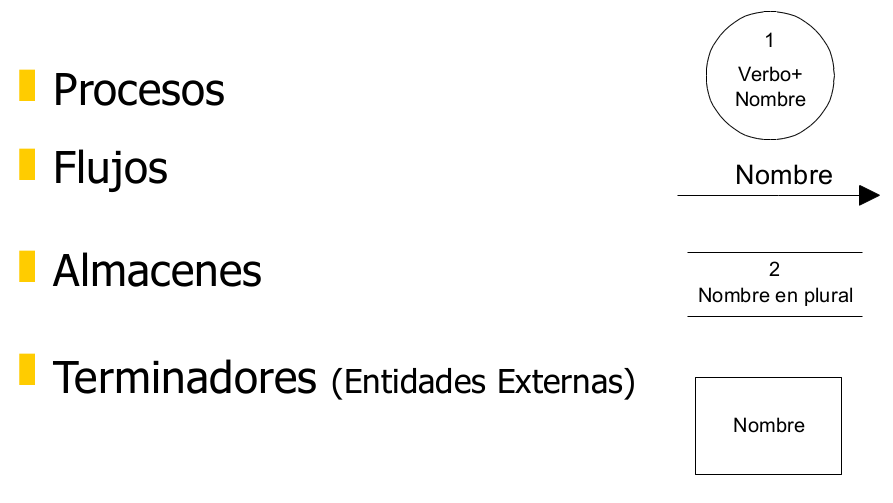
\includegraphics[width=\textwidth]{./images/dfds.png}
\end{figure}
%% o pantallazo con scrot(o)

Las \textbf{reglas} son:

\begin{itemize}[noitemsep]
\item Nombres con significado
\item Numerar los procesos NO implica secuencia
\item Evitar DFDs complejos
\item Todo DFD se redibuja varias veces
\end{itemize}

La \textbf{regla del balanceo} mantiene la consistencia entre las entradas y salidas de una burbuja padre y las entradas y salidas de todas sus burbujas hijas.

Para preservar la \textbf{consistencia lógica} de un Diagrama de Flujo de Datos hay que \textbf{evitar}:

\begin{itemize}[noitemsep]
\item Sumideros infinitos
\item Generaciones espontáneas
\item Flujos y procesos no etiquetados
\item Cuidado con los almacenes de sólo lectura o sólo escritura
\end{itemize}


\subsection{Diccionario de Datos} %% TODO
Un Diccionario de Datos es una \textbf{lista organizada} de todos los datos, que describe el \textbf{significado} y la \textbf{composición} de los flujos y almacenes, así como también las \textbf{relaciones} entre almacenes mediante un E/R.

Su \textbf{notación} es:

\begin{center}
  \begin{tabular}[h]{ l | l }
    \textbf{Símbolo}   & \textbf{Significado} \\
    \hline
    =                  & \textit{se define como} \\
    +                  & \textit{y} \\
    ()                 & opcional \\
    \{\}               & iteración \\
    \big[\big]         & separa alternativas \\
    *...*              & define datos elementales \\
    **                 & comentario \\
    @                  & identificador (clave) \\
    |                  & alternativa \\
  \end{tabular}
\end{center}

\subsection{Especificaciones de proceso}

Son sólo para los procesos (burbujas) de más bajo nivel. Se puede utilizar:

\begin{itemize}[noitemsep]
\item Lenguaje estructurado
\item Pre/post
\item Tablas de decisión
\item Gráficas
\item Lenguaje natural
\item Flow-charts
\end{itemize}

\textbf{Presentación por niveles}:

\begin{itemize}[noitemsep]
\item Los DFDs se presentan TOP-DOWN. Esto NO quiere decir que se construyan TOP-DOWN
\item El orden de presentación es: Diagrama de Contexto, Diagrama 0, Diagrama 1, etc...
\item ¿Hasta donde?: Se detiene la descomposición cuando las burbujas pueden especificarse como procesos sencillos (en menos de una página)
\item Sistemas sencillos: 2-3 niveles en total; medianos: 3-6; grandes: 5-8
\end{itemize}


\subsection{Entidad/Relación}

Las \textbf{entidades}:

\begin{itemize}[noitemsep]
\item Representan conjuntos de individuos
\item Cada individuo puede identificarse de manera única
\item Cada uno juega un papel necesario en el sistema
\end{itemize}

Yourdon no utiliza atributos en el diagrama pero sí en el Diccionario de Datos.

Las \textbf{relaciones} representan conjuntos de conexiones con sus cardinalidades.

Las \textbf{entidades asociativas} pueden verse como \textit{entidades que contienen los atributos de una relación}. Se utilizan para representar relaciones acerca de las cuales se quiere guardar alguna información. Como por ejemplo:

\textit{Un cliente compra artículos y queremos guardar información acerca del día y hora de la compra.}

En este caso ``Día'' y ``Hora'' serían \textbf{propiedades} de la relación, pero no de ``Cliente'' ni de ``Artículo''.

En el Diccionario de Datos tendríamos:

\begin{itemize}[noitemsep]
\item Cliente = @DNI + Nombre + Dirección + Telf.
\item Artículo = @Código + Descripción + Precio
\item Compra = @DNI + @Código + Día + Hora
\end{itemize}

A continuación se muestra un ejemplo de E/R con dos entidades
(Persona y Herramienta) y una relación (Usa):

\begin{center}
  \begin{tikzpicture}[node  distance =7em]
    \node[entity] (persona) {Persona};
    \node[relationship] (usa) [right  of=persona] {Usa} edge (persona);
    \node[entity] (herramienta) [right  of=usa] {Hrramienta} edge (usa);
  \end{tikzpicture}
\end{center}

Las reglas para la construcción de un modelo E/R son las siguientes:

\begin{itemize}[noitemsep]
\item Entrevistas, documentos: permiten la \textbf{identificación} de entidades
\item Se refinan y desarrollan en paralelo a los DFDs y DDs para mantener consistencia.
\item Simplificar:

  Eliminar objetos de instancia única

  Eliminar relaciones derivadas (calculables)

\item Regla heurística: si no somos capaces de imaginar al menos 3 registros de una entidad, malo.
\end{itemize}

\section{Relación entre notaciones}

\textbf{1. Diagrama de Flujo de Datos y Diccionario de Datos}

\begin{itemize}[noitemsep]
\item Todo flujo y almacén del DFD deben definirse en el DD y viceversa
\end{itemize}

\textbf{2. Diagrama de Flujo de Datos y Especificación de Proceso}

\begin{itemize}[noitemsep]
\item Toda burbuja del DFD debe asociarse con una burbija del nivel inferior, o con una especificación de proceso pero \textbf{no ambos}
\item Toda especificación de proceso debe asociarse a una burbuja de bajo nivel
\item Las entradas y salidas deben coincidir
\end{itemize}

\textbf{3. Especificación de Proceso con Diagrama de Flujo de Datos y Diccionario de Datos}

\begin{itemize}[noitemsep]
\item Los datos referenciados en la Especificación de Proceso deben coincidir con nombres de flujos o almacenes conectados a la burbuja, ser término local (variable local) o ser un componente del flujo o almacén
\end{itemize}

\textbf{4. Diccionario de Datos con Diagrama de Flujo de Datos y Especificación de Proceso}

\begin{itemize}[noitemsep]
\item Toda entrada del DD debe tener referencia en una Esp. Proc, un DFD o en el propio DD
\end{itemize}

\textbf{5. Entidad/Relación con Diagrama de Flujo de Datos y Especificación de Proceso}

\begin{itemize}[noitemsep]
\item Todo almacén del DFD debe corresponder a una entidad o entidad asociativa
\item Toda entidad, relación o entidad asociativa del E/R debe reflejarse en algún almacén del DFD
\item Los nombres deben coincidir: plural en DFD, singular en ER. Deben definirse ambas en el DD (ver a continuación)
\item Las instancias de las entidades y las relaciones del ER deben ser creadas o eliminadas por algún proceso
\item Alguna burbuja del DFD define valores para cada componente de datos
\item Alguna burbuja del DFD usa los valores de cada componente de datos
\end{itemize}

\textbf{6. Entidad/Relación: estensiones al Diccionario de Datos}

\begin{itemize}[noitemsep]
\item En general, las entidades se nombran en singular y los almacenes en plural
\item Los atributos de las entidades se pueden especificar en el DD
\end{itemize}

\section{Proceso de Construcción}

Consiste en elaborar los dos componentes del llamado \textit{Modelo Esencial}. Para lo que se construirá:

\subsection{Construcción del Modelo Ambiental}

\begin{itemize}[noitemsep]
\item Escribir en un párrafo el \textbf{propósito del sistema}
\item Construir el \textbf{diagrama de contexto} (preliminra identificando las entidades externas)
\item Construir una \textbf{lista de acontecimientos}
\end{itemize}

Una \textit{lista de acontecimientos} es una lista narrativa de los estímulos que ocurren en el mundo exterir a los cuales el sistema debe responder. Los hay de tres tipos:

\begin{itemize}[noitemsep]
\item \textbf{Flujo}: se asocian con la llegada de algún flujo
\item \textbf{Temporal}: se disparan a una determinada hora
\item \textbf{Control}: (no los tratamos)
\end{itemize}

\textit{Nota: los flujos y los acontecimientos son cosas distintas. No hay corrrespondencia uno-uno entre ambos.}

Los acontecimientos deben de contemplarse de fuera del sistema hacia dentro. Por ejemplo:

\textbf{Mal}: \textit{El sistema recibe el pedido del cliente}

\textbf{Bien}: \textit{El cliente hace un pedido}

La construcción de la \textit{lista de acontecimientos} se realiza \textbf{a partir} de las \textit{entidades externas}, pero el \textit{Diagrama de Contexto} se puede hacer \textbf{a la vez} que la \textit{Lista de acontecimientos}, se refinan mutuamente.

Los flujos del Diagrama de Contexto son el medio utilizado para la comunicación sistema-entorno. Los \textbf{flujos de entrada} son \textbf{utilizados} por los \textit{acontecimientos} y los \textbf{flujos de salida} son \textbf{respuestas} a los \textit{acontecimientos}.

\begin{itemize}[noitemsep]
\item Todo \textbf{acontecimiento no temporal} debe tener \textbf{entradas} para que el sistema pueda detectarlo.
\item Todo acontecimiento debe producir una \textbf{salida} inmediata y/o un \textbf{almacenamiento} de datos.
\end{itemize}


\subsection{Construcción de un Modelo de Comportamiento preliminar} %% TODO ejemplos

Consiste en desarrollar un \textit{Daigrama de Flujo de Datos} y un diagrama \textit{E/R} \textbf{preliminares}, además de las entradas iniciales del \textit{Diccionario de Datos}. Se opone al enfoque clásico debido a que \textbf{no es} top-down.

\begin{itemize}[noitemsep]
\item Se \textbf{dibuja} una burbuja o proceso por cada acontecimiento de la lista. El nombre de la burbuja describe la respuesta que se debe dar al acontecimiento.
\item Se \textbf{dibujan} las entradas, salidas y almacenes apropiados (conectados a la burbuja).
\item Se \textbf{conectan} las burbujas (de los acontecimientos) mediante almacenes.
\item En \textbf{paralelo} se contruye el diagrama \textit{E/R}.
\end{itemize}


\subsection{Acabado del Modelo}

\begin{itemize}[noitemsep]
\item Para finalizar el modelo se debe realizar una \textbf{Nivelación ascendente} hasta llegar al Diagrama de Contexto.

  - Los procesos o burbujas se agrupan por respuestas relacionadas.

  - Según se asciende se ocultan los almacenes internos a una agrupación de procesos. \textit{Sugerencia: hacer agregados de 7 +- 2 burbujas}.

\item Puede requerirse nivelación ascendente.
\item Completar el Diccionario de Datos
\item Completar la especificación del proceso(al final)
\item En \textbf{paralelo} acabar el diagrama E/R
\end{itemize}


\chapter{Objetos}
\label{chap:objetos}
% \setlength{\parindent}{4em}
% \setlength{\parskip}{1em}
%%% Local Variables:
%%% mode: latex
%%% TeX-master: "IS1apuntes"
%%% End:

\section{Orientación a objetos}
\label{sec:org3620eb4}
\subsection{Enfoque estructurado}
\label{sec:orgc590b61} Se denomina enfoque estructurado a la forma de
pensar el software en términos de funciones de transformación de datos
(se disocia entre funciones y datos, y las tareas se interpretan como
una transformación de los últimos).

\subsubsection{Ejemplo: Pintar un círculo}
\label{sec:orge1ddd3a} El enfoque estructurado resuelve el problema de
pintar un círculo de la siguiente forma:
\begin{itemize}
\item Usa una definición de círculo que esté acorde con los recursos
  de software (en este caso la expresión algebraica).

  \begin{equation} R^{2} \le (x - x_{0})^{2} + (y - y_{0})^{2}
  \end{equation}

  donde el radio R y las coordenadas del centro son las constantes que
  especifican un círculo concreto.
\item Disocia la definición de círculo en dos partes y las
  reinterpreta:
  \begin{itemize}
  \item Considera que R y el centro son datos para pintar el círculo y
    añade el color.
  \item Convierte la expresión declarativa en una función operativa
    que transforma el conjunto de datos precedentes en (x, y, color) de
    todos los píxeles para pintar el círculo en la pantalla.
  \end{itemize}
\item Como resultado final se obtiene un sistema capaz de pintar un
  círculo en términos de un proceso de transformación de datos.
\end{itemize}

El sistema software se expresa como una función F(x) que transforma el
conjunto de datos (R, x\(_{\text{0}}\), y\(_{\text{0}}\)) en otro
conjunto de datos, en este caso de píxeles.

\begin{figure}[ht!]  \centering
  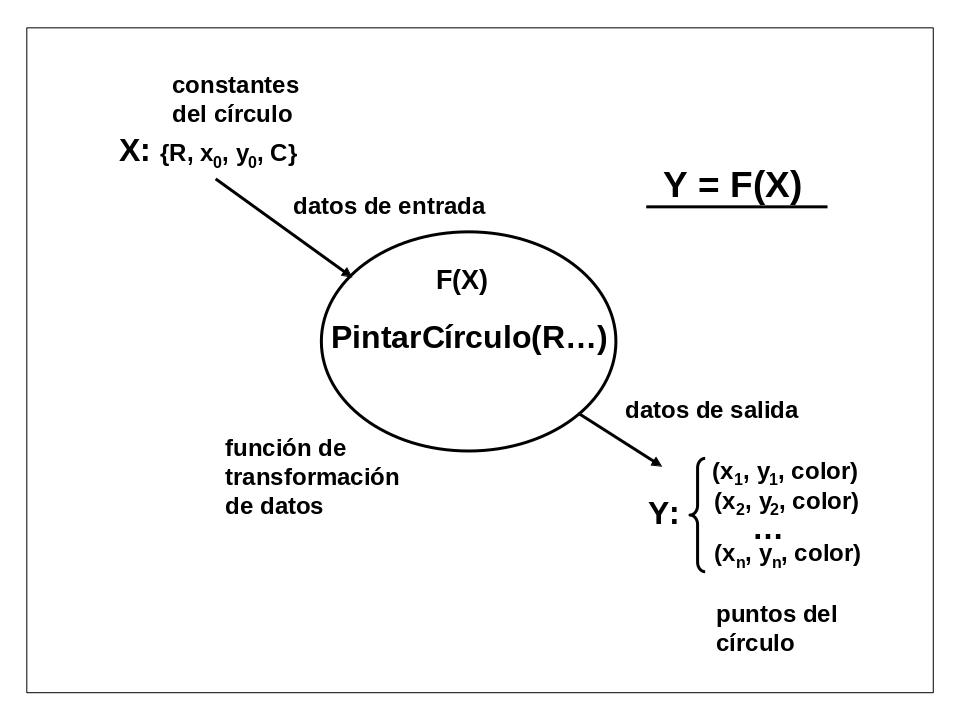
\includegraphics[width=0.5\textwidth]{images/fig12}
  \caption{Sistema software como función de transformación de datos}
  \label{fig:12}
\end{figure}

A este tipo de esquema se le denomina \emph{diagrama de flujo de
  datos}. \textbf{El diagrama de flujo de datos es un esquema asíncrono}
(no expresa secuencias); las flechas sólo indican los flujos de datos,
no el orden de ejecución.

\vspace{5mm}

El principal problema del enfoque estructurado es latente en el
momento en el que queremos añadir más elementos e interactuar con
ellos, por ejemplo, pintar varios círculos y actuar sobre los mismos
de forma selectiva, digamos borrar el segundo que se pintó.  Podríamos
hacer un bucle para crear n círculos, pero si queremos guardarlos
tendríamos que añadir tantas variables como círculos, con el objetivo
de retener cada conjunto de constantes. Este sistema es una
duplicación del sistema para solo un caso.

\vspace{5mm}

La disgregación de los conceptos en datos y funciones tiene sus pros y
sus contras, por ejemplo, este enfoque permite trabajar directamente
con la idea de base de datos o archivo, lo cual puede ser
beneficioso. Sin embargo, esta disociación implica \textbf{disminuir
  nuestro nivel de abstracción}.
\subsection{Enfoque orientado a objetos}
\label{sec:orgab1dc13} El enfoque orientado a objetos es la forma
particular de pensar el software en términos de elementos que
colaboran entre sí para realizar tareas.  Este enfoque nos da un nivel
de abstracción superior al estructurado, asociando cada elemento del
problema a un elemento software.  Cada elemento software tiene las
propiedades íntegras de cada elemento del discurso (lo que \emph{hace
  a una cosa ser una cosa}).
\subsubsection{Ejemplo: Pintar un círculo}
\label{sec:orge1a8962} En el ejemplo anterior, definimos un objeto
\texttt{círculo} que cumple las propiedades de un círculo según la
definición que hemos adaptado para nuestro sistema (en este caso, el
objeto contiene un centro y un radio) y tiene los mecanismos para
pintarse y crearse como elemento.

El enfoque de objetos piensa:
\begin{itemize}
\item En variables software capaces de recordar las constantes de un
  círculo, capaces de pintar un círculo y capaces de crearse a sí mismas
  como variables.
\item En el sistema software en términos de la interacción de estas
  variables, dadas sus respectivas capacidades para ejecutar
  operaciones, es decir, cómo relacionar todas las variables para
  conseguir que se realice la tarea de pintar círculos.
\end{itemize}

\begin{figure}[ht!]  \centering
  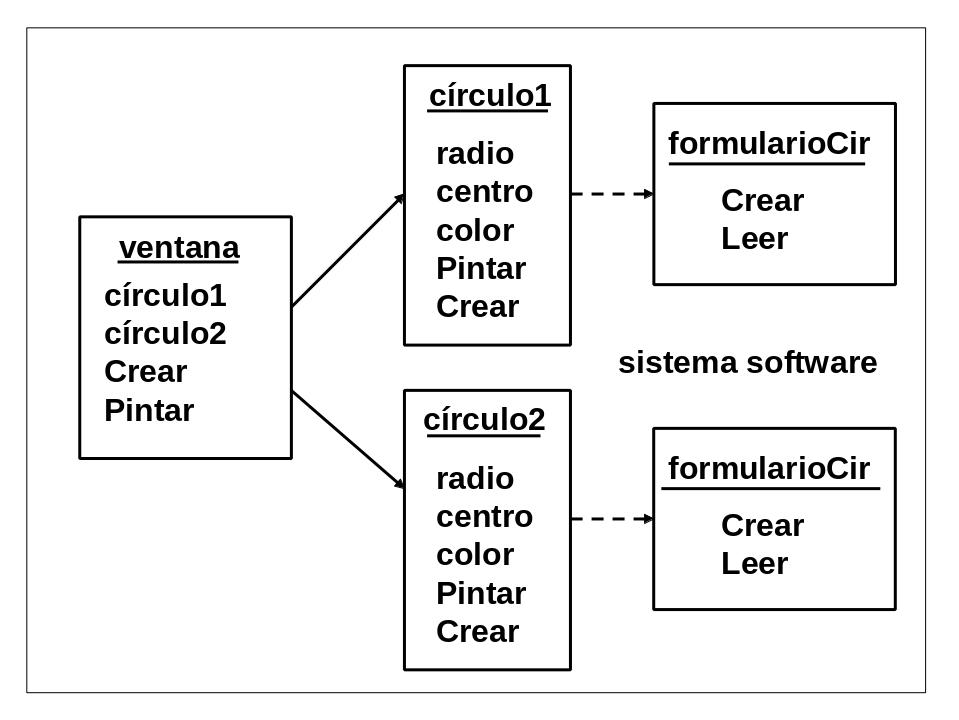
\includegraphics[width=0.5\textwidth]{images/fig18}
  \caption{Sistema software con enfoque de objetos}
  \label{fig:18}
\end{figure}

Este esquema muestra el sistema software, donde se aprecian las
relaciones entre las variables software que ejecutan la tarea de
pintar un círculo.  Como vemos, el sistema software, aun aplicando el
mismo algoritmo, tiene una organización diferente, y por tanto sus
propiedades también varían.
\subsection{Objetos}
\label{sec:org2b984f4} Esto que hemos ido llamando \emph{variables
  software} se conocen en este enfoque como \textbf{objetos}, y amplían
la idea de la variable software tratada en el enfoque estructurado, ya
que tienen capacidad de expresar cualquier cosa, incluso operaciones.
Otra definición complementaria de objeto es la siguiente: \emph{Un
  objeto es un elemento software cualitativamente distinto capaz de
  expresar un concepto más amplio, más ambiguo: cosa.}

\vspace{5mm}

Los objetos interactúan entre ellos mediante \textbf{mensajes},
solicitudes a objetos para que ejecuten operaciones.  Una buena
analogía de objetos y mensajes es el teatro, los objetos son
\emph{actores} y los mensajes son \emph{su diálogo}; el programa
describe a los actores, lo que tienen que hacer y decir.

\subsubsection{Propiedades de los objetos} Los objetos son definidos
por su nombre, asociado con una dirección de la memoria de la máquina.
Esta definición puede considerar además las propiedades que,
generalmente, se clasifican en \emph{atributos y operaciones}, también
denominadas \emph{métodos}.
\begin{itemize}
\item \textbf{Atributo:} Propiedad de un objeto, que está compuesto
  por un objeto o por una variable software tradicional. Los lenguajes
  OOP puros (como SmallTalk) solo admiten objetos como atributos, pero
  los lenguajes híbridos (como Java) también admiten variables software
  tradicionales.
\item \textbf{Operación: } Propiedad de un objeto que expresa su
  capacidad para ejecutar la rutina indicada por la misma. Las
  operaciones representan cualquier código capaz de ejecutar acciones.
\end{itemize}

\vspace{5mm}

Los lenguajes de programación acostumbran a distinguir los atributos
de las operaciones para elevar la eficiencia de compilación, pero en
principio, \textbf{no hay razón para distinguirlos}.

\vspace{5mm}

\paragraph{Globalidad de los atributos y operaciones:} Los atributos
de un objeto son globales para todas las operaciones del mismo. Esto
es, cualquier línea de código de cualquier método de un objeto tiene
acceso inmediato a todos los atributos del propio objeto. Esto
facilita el acceso a los atributos, pero tiene los siguientes
inconvenientes:
\begin{itemize}
\item Cuando una operación de un objeto quiere usar otra operación del
  mismo, esta operación no conoce cómo usarla, ya que en la cabecera de
  la operación llamada no se refleja la relación con los atributos del
  objeto, y podría interceder en el uso de los atributos de la operación
  llamante.
\item Al modificar alguna línea de código de una operación debemos
  revisar todas las líneas de código de todas las operaciones, ya que
  cambiar el comportamiento de una operación que a priori puede ser
  necesaria para el resto de operaciones podría desencadenar en un mal
  funcionamiento del objeto.
\end{itemize}

\vspace{5mm}

\paragraph{Visibilidad de los atributos y operaciones:} Los objetos
son, de una forma coloquial, \emph{parcelas bien definidas};
accesibles desde dentro pero no tan fácilmente desde fuera. El acceso
desde fuera está regulado por un "control de visibilidad".
Los elementos designados como \emph{públicos} son accesibles a todos
los objetos del sistema software. Los \emph{privados} son accesibles
sólo desde el propio objeto.

\subsubsection{Sobre la ambigüedad} Una de las característica más
importantes del enfoque orientado a objetos es la capacidad de éstos
para expresar alternativas o significados diversos, lo que comúnmente
llamamos \textbf{ambigüedad}.

\vspace{5mm}

El enfoque estructurado utiliza dato y función de transformación de
datos como elementos del sistema software, mientras el enfoque de
objetos utiliza los elementos objeto, con el significado de
\emph{cosa}, y mensaje con el significado de solicitud de servicio a
una variable.  El significado ambiguo de \emph{cosa} que tienen los
objetos nos permite hacer un diseño estructurado con aspecto (ropaje?)
de objetos, pero no al contrario (diseño de objetos con aspecto
estructurado).

\vspace{5mm}

\textbf{El enfoque de objetos se acomoda mejor a la diversidad de
  problemas que aborda el software.}  Los objetos son más tolerantes
para expresar la idea general de función que el enfoque estructurado,
el cual está obligado a expresar esa función en términos de “entrada,
proceso y salida”.  No obstante, esta mayor libertad de expresión
tampoco es gratis siempre. A menudo hay que aceptar cualidades
“extrañas” como la capacidad de pintarse, ampliarse, moverse,
borrarse, etc.  que tienen los círculos software, para ajustarse al
enfoque.

\vspace{5mm}

La \textbf{ambigüedad del enfoque de objetos} también facilita que un
\textbf{elemento software}, por sí solo, \textbf{exprese completamente
  un concepto}, por ejemplo círculo, mientras que el enfoque
estructurado obliga, muchas veces, a disociarlos en funciones y datos.


\begin{figure}[ht!]  \centering
  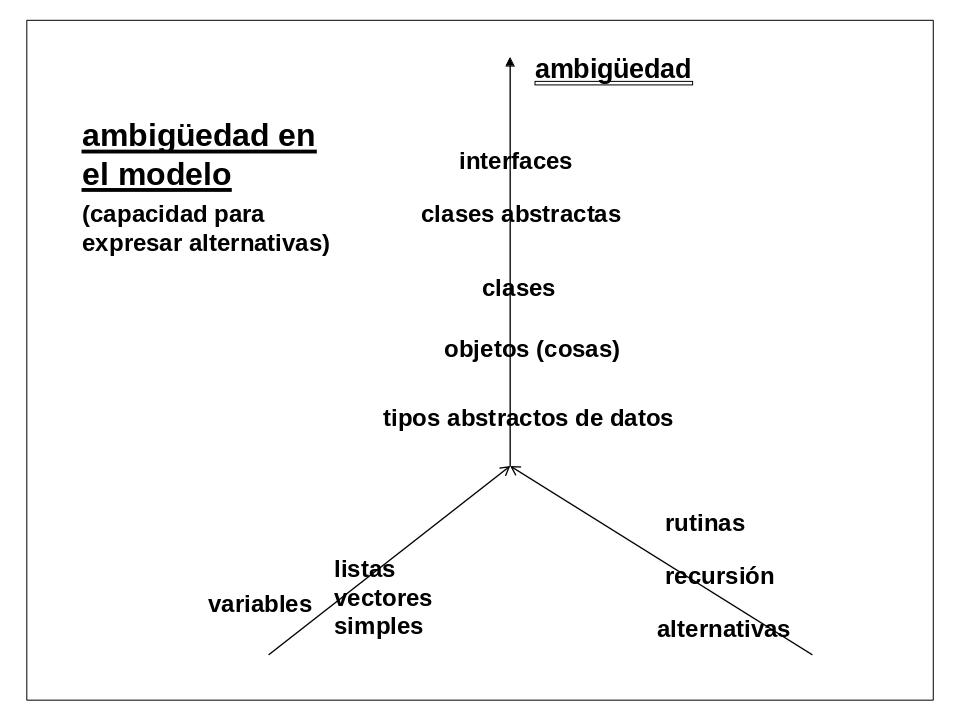
\includegraphics[width=0.5\textwidth]{images/fig111}
  \caption{Aumento de la capacidad de ambigüedad en elementos
    software}
  \label{fig:111}
\end{figure}

La figura muestra la evolución del software hacia el aumento de la
ambigüedad de sus elementos primarios.  También nos muestra claramente
qué es un TAD, es decir, un \emph{tipo abstracto de datos}. Estos TAD
\textbf{no se consideran objetos}, ya que, a diferencia de éstos,
siempre deben ser datos (un objeto no tiene por qué ser un dato, puede
ser cualquier cosa, no está comprometido a desempeñar dicha función ni
ninguna en particular).

\subsubsection{Objetos vs Realidad} Gracias a la mayor capacidad
expresiva de los objetos se dice a menudo que los objetos reflejan
mejor la realidad.  Pero esta idea perjudica, más que beneficia porque
reflejar la realidad:
\begin{itemize}
\item No es el propósito de los sistemas software, salvo que sean de
  simulación.
\item Dificulta los cambios en los sistemas software.
\item ¿Qué significa? La realidad varía según el espectador.
\end{itemize}

\subsubsection{Refactorización}
Se llama \emph{refactorización} a los procesos que \textbf{modifican
  el sistema para mejorar alguna cualidad interna sin alterar sus
  funciones}. A diferencia de la forma tradicional, que aspira
a alcanzar un diseño perfecto, la refactorización acepta que el
objetivo es funcionar a tiempo, y que después de probarlo se podrá
mejorar el funcionamiento del sistema software.

\subsubsection{Encapsulado y principio de ocultación}
Como un objeto es una \emph{parcela de software}, se suele decir que
un objeto \textbf{encapsula} sus atributos y operaciones, lo cual es
correcto, no distorsiona nuestra analogía con la parcela. No obstante,
cuando se asocia encapsulado con ocultación de información tenemos un
problema.\\
Es cierto que el enfoque de objetos facilita algunas formas de
desarrollo de software, como los prototipos evolutivos y el diseño en
paralelo, pero no son facilidades intrínsecas.\\
\textbf{El principio de ocultación establece que:}
\begin{itemize}
\item Cada módulo es independiente del código de la implementación
  de los demás (los clientes se comunican con los servicios por
  medio de interfaces, que permiten realizar las operaciones sin
  conocimiento de la modificación del código anteriormente
  mencionado).
\item La interfaz o definición de cada módulo debe revelar lo menos
  posible del trabajo interno del módulo.
\end{itemize}

\newpage

\subsection{Representación gráfica de los objetos}
En este apartado veremos varios tipos de gráficos para representar
objetos, sus atributos, operaciones y la interacción entre ellos (es
decir, los mensajes).
\subsubsection{UML (Unified Modelling Language)}
UML es un sistema de símbolos y diagramas (un lenguaje) que sirve para
expresar (modelar) los diseños de los sistemas software. La palabra
unificado refleja el acuerdo de sus autores.

\paragraph{Objetos:}
UML representa a los objetos mediante \textbf{cajas}. Si se usa la
definición extendida de objeto, la caja marca tres zonas: la superior
contiene, subrayado, el nombre del objeto; la zona central contiene
los atributos y la inferior los métodos u operaciones. En caso de usar
la definición compacta de objeto, la caja solo contiene la zona
superior. En UML los elementos públicos son diferenciados de los
privados según el símbolo que precede su nombre; \textrm{+} para los públicos
y \textrm{-} para los privados.

\begin{figure}[ht!]  \centering
  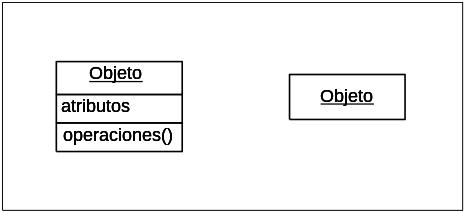
\includegraphics[width=0.5\textwidth]{images/fig21}
  \caption{Representación de un objeto en UML}
  \label{fig:21}
\end{figure}

\vspace{5mm}

\paragraph{Mensajes:}
UML representa los mensajes mediante líneas dirigidas etiquetadas con
el nombre de su operación, \textbf{desde el llamante al llamado}.

\begin{figure}[ht!]  \centering
  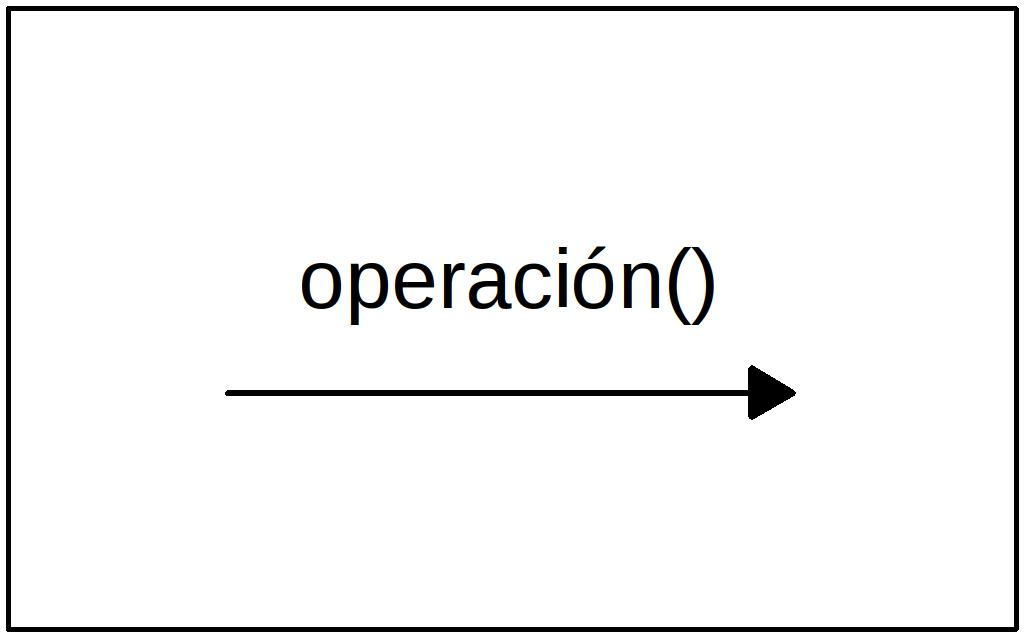
\includegraphics[width=0.3\textwidth]{images/fig22}
  \caption{Representación de un mensaje en UML}
  \label{fig:22}
\end{figure}

\paragraph{Diagrama de secuencias:}
Los objetos que participan en la interacción se dibujan,
horizontalmente, en la parte superior del diagrama a través de sus
esquemas simplificados (cajas conteniendo sólo el nombre
subrayado). Debajo de cada objeto se dibuja una línea vertical
discontinua llamada línea de vida que indica, en el eje tiempo, la
existencia del objeto.
Los mensajes se colocan entre las líneas de vida de los objetos,
siguiendo la secuencia de ejecución. Si se quiere resaltar la
devolución de algún valor, se puede dibujar una flecha discontinua
apuntando hacia el objeto emisor, etiquetada con el nombre del valor
de retorno.

\begin{figure}[ht!]  \centering
  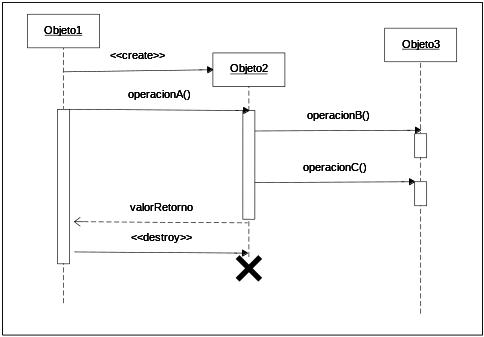
\includegraphics[width=0.5\textwidth]{images/fig23}
  \caption{Diagrama de secuencias en UML}
  \label{fig:23}
\end{figure}

Para indicar la creación o destrucción de un objeto se utilizan,
respectivamente, las etiquetas estereotipadas \textrm{<<create>>} y
\textrm{<<destroy>>} en el mensaje que se le envía al objeto. La
creación de un objeto se distingue dirigiendo el mensaje a la caja que
representa al objeto. La destrucción de un objeto se muestra dibujando
una X grande al final de su línea vida.
\newpage
\paragraph{Diagrama de colaboración:}
Un diagrama de colabroación e sun diagrama de interacción que resalta
la organización de los objetos que envían y reciben los mensajes. Este
diagrama muestra un conjunto de objetos, los enlaces entre ellos y los
mensajes que intercambian.\\
\textbf{Un enlace es una instancia de una asociación o dependencia entre
  clases.} Se representa con una línea continua que une los dos
objetos.

\begin{figure}[ht!]  \centering
  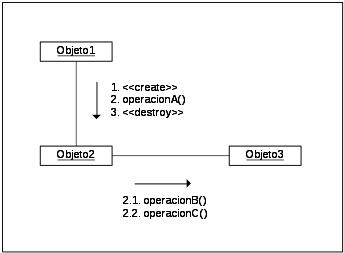
\includegraphics[width=0.5\textwidth]{images/fig25}
  \caption{Diagrama de colaboración en UML}
  \label{fig:25}
\end{figure}

Los mensajes se escriben junto a los enlaces, indicando el sentido con
una flecha que apunta hacia el receptor y numerándolos para expresar
el orden de ejecución. \\
El diagrama de colaboración ofrece una vista de conjunto de estructura
y funcionamiento, pero incide en la estructura, afectando a la
claridad del funcionamiento (toca seguir la secuencia de mensajes
saltando de una línea a otra, buscando la numeración).\\
Además, esta forma de representación dificulta la modificación del
diseño, por lo que interesa usar este diagrama cuando no interese
demasiado seguir el funcionamiento y se esperen pocas modificaciones
del diseño.

\subsection{Clases}
Una \textbf{clase} es una definición intensiva de un conjunto de
objetos. Establece las propiedades distitntivas de cualquier elemento
del conjunto que define.\\

\vspace{5mm}

Considerando las clases se podría decir que un objeto es una
\textbf{instancia} de una clase o un elemento del conjunto definido
por una clase. La notación UML de un objeto en particular, teniendo en
cuenta la clase a la que pertenece, es \texttt{objeto:clase}. Si se
quiere expresar un objeto cualquiera (anónimo) de una clase, la
notación sería \texttt{:clase}.

\vspace{5mm}

Las clases enriquecen el enfoque de objetos. Un objeto es una cosa y
una clase define un conjunto de cosas con iguales propiedades, pero
valores distintos, por tanto las clases establecen una generalización,
una \textbf{abstracción} mayor que los objetos. La \textbf{estructura y
relaciones de los elementos del sistema} software se pueden pensar en
términos de las \textbf{clases}, y dejar los objetos para pensar los diseños
dinámicos particulares del sistema.

\vspace{5mm}

La representación de las clases y los objetos coinciden prácticamente
en el lenguaje UML, con la salvedad de que el nombre de las clases no
se subraya.

\subsubsection{Diagrama de clases}
El diagrama de clases expresa la estructura u organización del sistema
software en términos de las clases. Además de intervenir en el
funcionamiento, el diseño del diagrama es clave porque expresa la
organización del sistema, y ésta decide sobre aspectos fundamentales:
significado, facilidad de desarrollo en paralelo y faciidad de modificación.

\begin{figure}[ht!]  \centering
  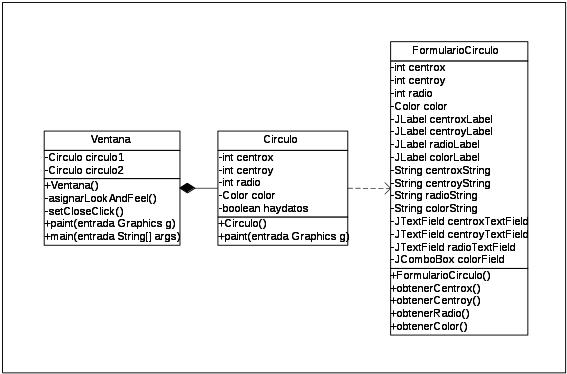
\includegraphics[width=0.5\textwidth]{images/fig33}
  \caption{Diagrama de clases en UML}
  \label{fig:33}
\end{figure}

La figura muestra el diagrama de clases del sistema para dibujar
círculos. Se aprecian las clases, los elementos que componen cada
clase y las relaciones entre las clases, así como la visibilidad de
dichos elementos.\\
El diagrama de clases complementa a los diagramas de secuencias,
muestra la forma del soporte de los mecanismos, mientras que los
diagramas de secuencias muestran el funcionamiento parcial de los
mecanismos.
\begin{figure}[ht!]  \centering
  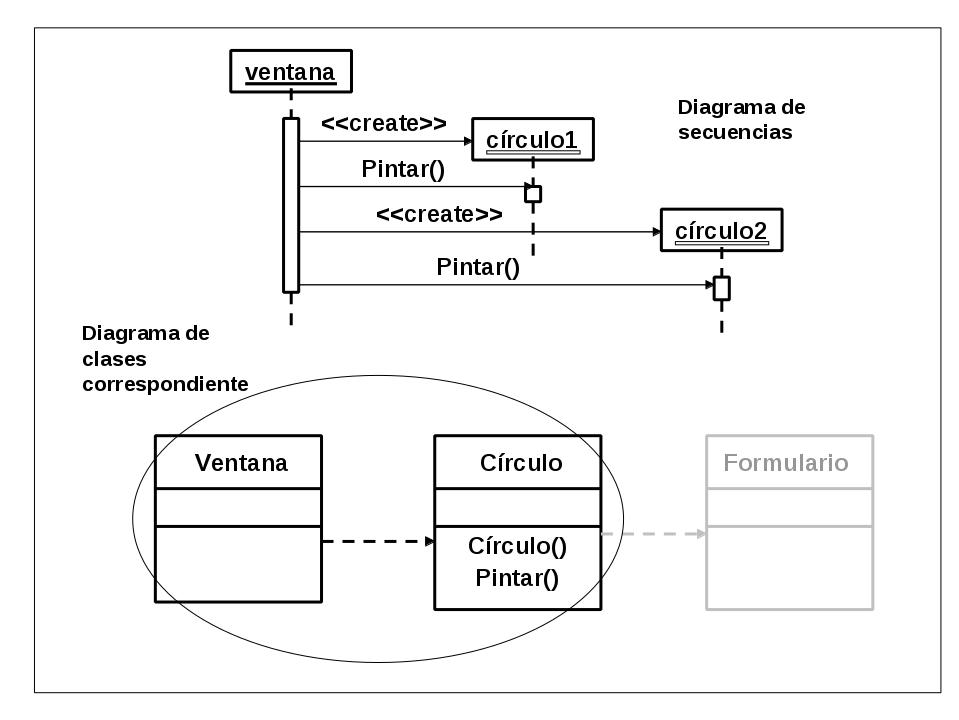
\includegraphics[width=0.5\textwidth]{images/fig34}
  \caption{Correspondencia entre diagrama de clases y de secuencia en UML}
  \label{fig:34}
\end{figure}

\chapter{Arquitectura}
\label{chap:arquitectura}
%%% Local Variables:
%%% mode: latex
%%% TeX-master: "IS1apuntes"
%%% End:

\section{Introducción a la arquitectura}
\label{sec:arquitectura:intro}

Requerimientos \textrightarrow Diseño \textrightarrow Construcción
\textrightarrow Pruebas \textrightarrow Implantación.
\\

La arquitectura de Software de un sistema es el \textbf{conjunto} de 
\textbf{estructuras} necesarias para \textbf{razonar} sobre el
sistema. Relaciona distintos elementos de software como son los
objetos o los hilos de ejecución; el modelo del sistema,
los diagramas, la lógica; o las entidades físicas como los nodos donde
se ejecutará Software.

Desde una perspectiva de alto nivel, la arquitectura de Software cubre
diferentes componentes del sistema. Tendrá en cuenta los
requerimientos y fines del sistema, pero a la vez la creación del
modelo, las dependencias y los escenarios de uso. Es decir, la
arquitectura de software maneja sin encargarse de la implementación
final, los aspectos técnicos y de uso que ocurrirán durante el
desarrollo del sistema. Crea por tanto una estructura orientada al
rendimiento, usabilidad y modificabilidad (\textbf{requisitos de calidad}).

\section{Requerimientos}
\label{sec:arquitectura:requerimientos}

Objectivos de negocio\textrightarrow Drivers arquitectónicos
\textrightarrow Decisiones arquitectura\textrightarrow\\ Arquitectura
documentada\textrightarrow Riesgos Deudas
\\\par
Un requerimientos es una \textbf{especificación} que describe alguna
funcionalidad, atributo o factor de calidad de un sistema software.
\\\par
Requerimiento\textrightarrow Diseño\textrightarrow Documentación
\textrightarrow Evaluación\textrightarrow Implementación

Existe una amalgama de intereses y requerimientos entre los distintos
actores que usarán el sistema. Si bien todos juegan un papel
fundamental, a nivel de equipo de desarrollo se deberán satisfacer los
requerimientos funcionales, es decir, usar una \emph{combobox} para
elegir los billetes.\cite[p.~14]{IS1ArquitecturaDia1}

La \textbf{ISO 9126} ofrece una descripción de los criterios de
calidad del software (sección \ref{sec:cv}):\index{ISO
  9126}\index{criterios de calidad}

\begin{itemize}[noitemsep]
\item Funcionalidad
\item Confiabilidad
\item Usabilidad
\item Eficiencia
\item Mantenibilidad
\item Portabilidad
\end{itemize}

Los \textbf{drivers} son un subconjunto de requerimientos que definen
la estructura de un sistema. Existen los drivers \textbf{funcionales},
\textbf{de atributos de alta calidad}, y los drivers de
\textbf{restricciones}.\index{drivers}

\begin{description}
\item[Funcionales] Descomposición del sistema. Relevancia y
  complejidad.
\item[Calidad] Los atributos de calidad.
\item[Restricciones] Técnicas y de gestión.
\end{description}
\label{sec:drivers}

\subsubsection{Métodos para identificar drivers arquitectónicos}
\label{sec:drivers}

Existen diferentes métodos para identificar drivers
arquitectónicos. Podemos basarnos en \emph{talleres de atributos},
métodos de diseño o \emph{FURPS}.\index{talleres de atributos}

El propósito de los talleres de atributos es ayudar a elegir la
arquitectura adecuada para un sistema de Software. El modelo
\emph{QAW} (Talleres de calidad del Atributo) se centra en los
requisitos del cliente, y no hace necesaria la existencia previa de
una arquitectura software.\index{QAW}

\section{Diseño de estructuras}
\label{sec:arquitectura:diseñoestructura}

El diseño es la especificación de un \textbf{objeto}, creado por algún
\textbf{agente}, que busca alcanzar ciertos \textbf{objectivos}, en un
\textbf{entorno} particular, usando un conjunto de
\textbf{componentes} básicos, satisfaciendo una serie de
\textbf{requerimientos} y sujetándose a determinadas
\textbf{restricciones}.

\begin{center}
  \textit{Teniendo en cuenta lo que nos han pedido, juntar piezas que
    tenemos teniendo en cuenta nuestras restricciones para describir lo que queremos
    hacer.}
  Arquitectura\textrightarrow Interfaces\textrightarrow Detalle de los módulos
\end{center}

Se diseña en base a los principios de \textbf{modularidad},
\textbf{alta cohesión y bajo acomplamiento} y de \textbf{mantener las
  cosas simples}.

Los patrones de diseño juegan un papel fundamental en la espeficiación
de los drivers.\index{patrones de diseño} Se abstraen problemas ya
resueltos sin llegar a representar soluciones detalladas para luego
adaptarlo a cada caso particular. Cuando los diseños son más
concretos, se llegan a crear elementos software reutilizables que
proporcionan la funcionalidad genérica enfocándose a la resolución de
un problema específico. Así nacen los \textbf{frameworks}\index{framework}.

A la hora de diseñan las \textbf{interfaces} se identifican los
mensajes que se intercambian.\index{interfaces}

\section{Diseño de Arquitecturas}
\label{sec:arquitectura:diseñoarquitectura}

El problema del diseño de la arquitectura se resuelve mediante diseños
\textbf{basados en atributos}, \textbf{centrados en arqutectura} o con
\textbf{vistas y perspectivas}. El método de \textbf{Rozansky \&
  Woods}.\index{ADD}\index{ACDM}\index{Rozansky \& Woods}


\begin{figure}[h]
  \centering
  \begin{tabular}[h]{p{2.5cm} || p{3cm} | p{3cm} | p{5cm}}
    &\textbf{ADD}&\textbf{ACDM}&\textbf{Rozansky \& Woods} \\ \hline
    Mecánica y enfoque & Diseño iterativo descomponiendo elementos
                         recursivamente & Iteraciones de diseño,
                                          documentación y
                                          evaluación. & Iteraciones de diseño,
                                                        documentación y
                                                        evaluación. \\
    Participantes & Arquitecto & Arquitecto y otros & Arquitecto y
                                                      otros \\
    Entradas & Drivers & Drivers y alcance & Vistas \\
    Salidas & Esbozos de vistas & Vistas & Vistas \\
    Criterios de terminación & Se satisfacen los drivers & Los
                                                           experimentos
                                                           no revelan
                                                           riesgos o
                                                           son
                                                           aceptables
                               & Los interesados están de acerudo en
                                 que el diseño satisface sus
                                 preocupaciones. \\
    Conceptos de diseño utilizados & Técnicas y patrones & Estilos
                                                           arquitectónicos,
                                                           patrones y
                                                           prácticas &
                                                                       Estilos
                                                                       arquitectónicos
                                                                       y patrones.
    \end{tabular}  
  \caption[Comparación diseño arquitecturas]{Comparación de métodos de
    dieseño de arquitecturas}
  Interesante ver la figura \ref{fig:costemetodologia}
  \label{fig:comparaciondiseñoarquitectura}
\end{figure}


\section{Documentación}
\label{sec:documentacion}

\begin{center}
  \textit{Generación de documentos que describen las estructuras de la
  arquitectura con el propósito de comunicar efectivamente a los
  interesados en el sistema.}
\end{center}

La documentación se apoya en vistas para la descripción de las
estructuras. Se componen de un diagrama que representa los objetos de
la estructura y de información textual que ayuda a comprender el
diagrama.

\index{vista lógica}La \textbf{vista lógica} representa en el diagrama
\emph{unidades} de implementación, que pueden ser en base a la
funcionalidad o la responsabilidad.

Otras \emph{vistas} son las de \textbf{comportamiento}, las \textbf{físicas}
o la de Windows\texttrademark~\footnote{Que no nos gusta.}.

\section{Evaluación}
\label{sec:arquitectura:evaluacion}

\begin{center}
  \textit{La evaluación es la técnica para evitar que los defectos lleguen a
  los usaurios finales o que se presenten en momentos donde
  corregirlos sea complicado.}
\end{center}

La evaluación sirve para determinar si el software cumple con los
criterios de calidad (\ref{sec:software}). Al evaluar un sistema se
pueden producir \emph{desviaciones} respecto a las necesidades de los
usuarios o respecto a la construcción correcta del producto. Al
evaluar las arquitecturas se busca satisfacer los drivers
arquitectónicos (\ref{sec:drivers}).

\section{Implementación}
\label{sec:implementacion}

La implementación busca generar diseños detallados de los módulos y
otros elementos siempre de acuerdo con la arquitectura. Se ajustan los
diseños y errores, pero no se cambia la arquitectura.

\begin{itemize}[noitemsep]
\item Diseñar la estructura del sistema basándose en la arquitectura.
\item Basarse en los requisitos funcionales (\ref{sec:drivers}).
\item Desarrollar\footnote{Picar código y fixes.}.
\end{itemize}

La resolución de las desviaciones (\emph{errores}) se resuelve
mediante controles de calidad en los que se \textbf{verifica el
  código}, el \textbf{diseño}. Además de realizar \textbf{pruebas} y
\textbf{auditorías}.

%%% Local Variables:
%%% mode: latex
%%% TeX-master: "IS1apuntes"
%%% End:
\section{Arquitectura Software}
\label{sec:arquitectura:arquitectura}


\begin{description}
\item[Componente] Bloque del sistema. Parte que combinas con la arquitectura.
\item[Servicio] Funcionalidad que los componentes proporcionan a los actores.
\end{description}

Al dividir un sistema en componente, hay que definir los servicios que
proporciona cada componente.

\subsection{Estilos}
\label{sec:estilos}

El estilo es la forma general de un sistema, semejante a lo que serían
los patrones de diseño (\ref{sec:arquitectura:diseñoestructura}). Al
definir un estilo, se deben especificar los elementos como los bloques
básicos de contrucción, las conexiones entre los bloques y las reglas
que espeficican cómo se combinan los servicios.

\begin{figure}[h]
  \centering
  \begin{tabular}{l | l}
    \textbf{Técnica}&\textbf{Patrón}\\\hline
    Abstracción&Niveles \\
    Encapsulación & Expedidor-receptor \\
    Ocultación de información&Reflexión, Composite \\
    Modularización&Niveles, Pipes \& Filters, Composite\\
    Acoplamiento y
    cohesión&Publicador-Suscriptor,Cliente-Despachador-Servidor\\
    Separación de intereses&Modelo-Vista-Controlador
  \end{tabular}
  \caption{Patrones que ayuan a aplicar técnicas}
  \label{fig:patronesestilo}
\end{figure}

\subsection{Índice de un documento de arquitectura}
\label{sec:indicearquitectura}
\begin{itemize}[noitemsep]
\item Objetivos
\item Requerimientos (\emph{funcionales, no funcionales})
  (\ref{sec:arquitectura:requerimientos})
\item Decisiones y justificación
\item Modelo conceptual (\ref{sec:documentacion})
  \begin{itemize}[noitemsep]
  \item Modelo de componentes lógicos
  \item Modelo de procesos
  \item Modelo físico
  \item Modelo de despliegue
  \end{itemize}
\item Despliegue de la arquitectura
\end{itemize}

Otra información relevante del documento de arquitectura es presentar
distintos diagramas:
\begin{itemize}[noitemsep]
\item Diagrama de Clases (\emph{Lógica}).
\item Diagrama de Paquetes (\emph{Desarrollo}).
\item Diagrama de Interacción (\emph{Procesos}).
\item Diagrama de Despliegue (\emph{Física}).
\end{itemize}

\subsubsection{Pasos en la identificación de un problema}
Metas del proceso\textrightarrow Recogida de
información\textrightarrow Conceptos de la Arquitectura\textrightarrow
Cliente de la solución\textrightarrow Definición del problema

\subsection{Patrones}
\label{sec:patrones}

\begin{enumerate}[noitemsep]
\item Especificar el problema.
  \begin{itemize}[noitemsep]
  \item Dividir el problema.
  \item Encontrar el contexto.
  \item Considerar pros/cons.
  \item Acceder al catálogo de patrones.
  \end{itemize}
\item Seleccionar la categoría de los patrones (\emph{arquitectónicos
  o de diseño}).
\item Categoría del problema.
\item Comparar descripciones del problema.
\item Comparar beneficios y compromiso.
\item Elegir la mejor variante.
\end{enumerate}

Entre los ejemplos de patrones están: \emph{N-Niveles, Filtros y
  Tuberías, Pizarra, Modelo-Vista-Controlador}.

\chapter{Apéndices}
\section{Examen Junio 2009}
\begin{figure}
  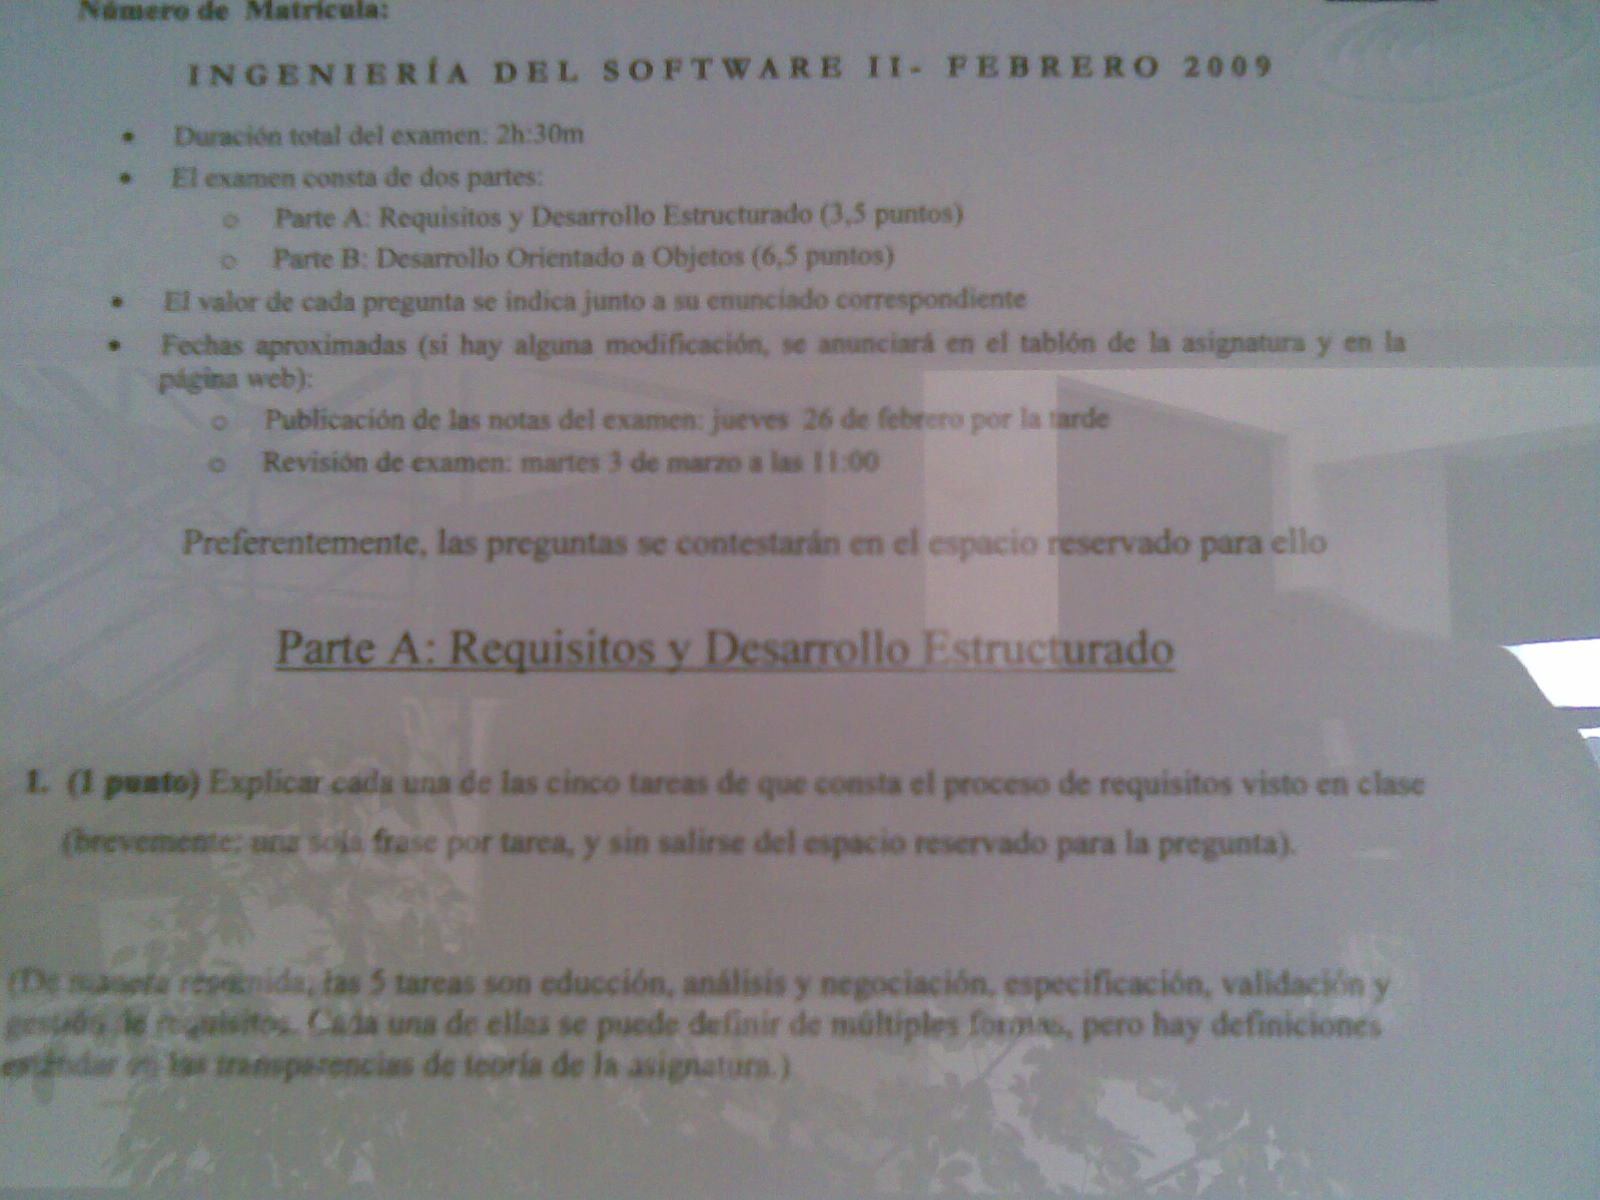
\includegraphics[width=\textwidth]{./images/jun/Imagen072.jpg}
\end{figure}
\begin{figure}
  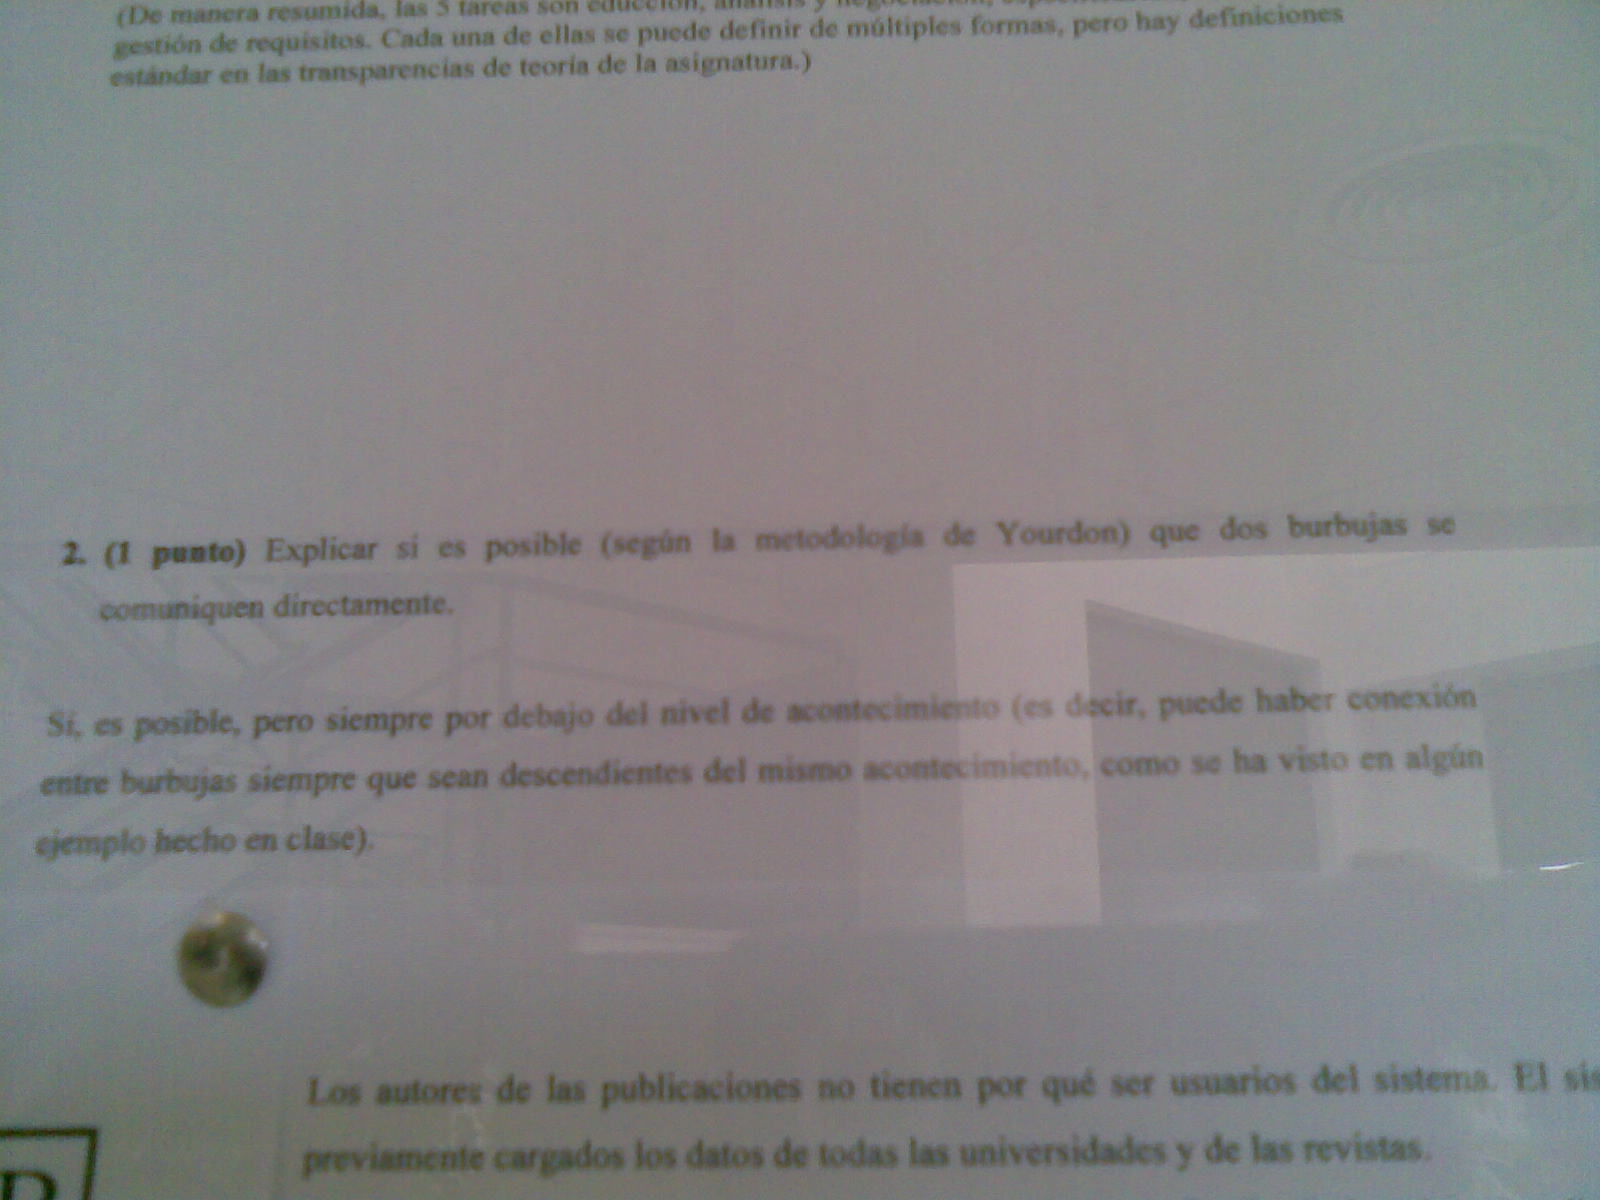
\includegraphics[width=\textwidth]{./images/jun/Imagen074.jpg}
\end{figure}
\begin{figure}
  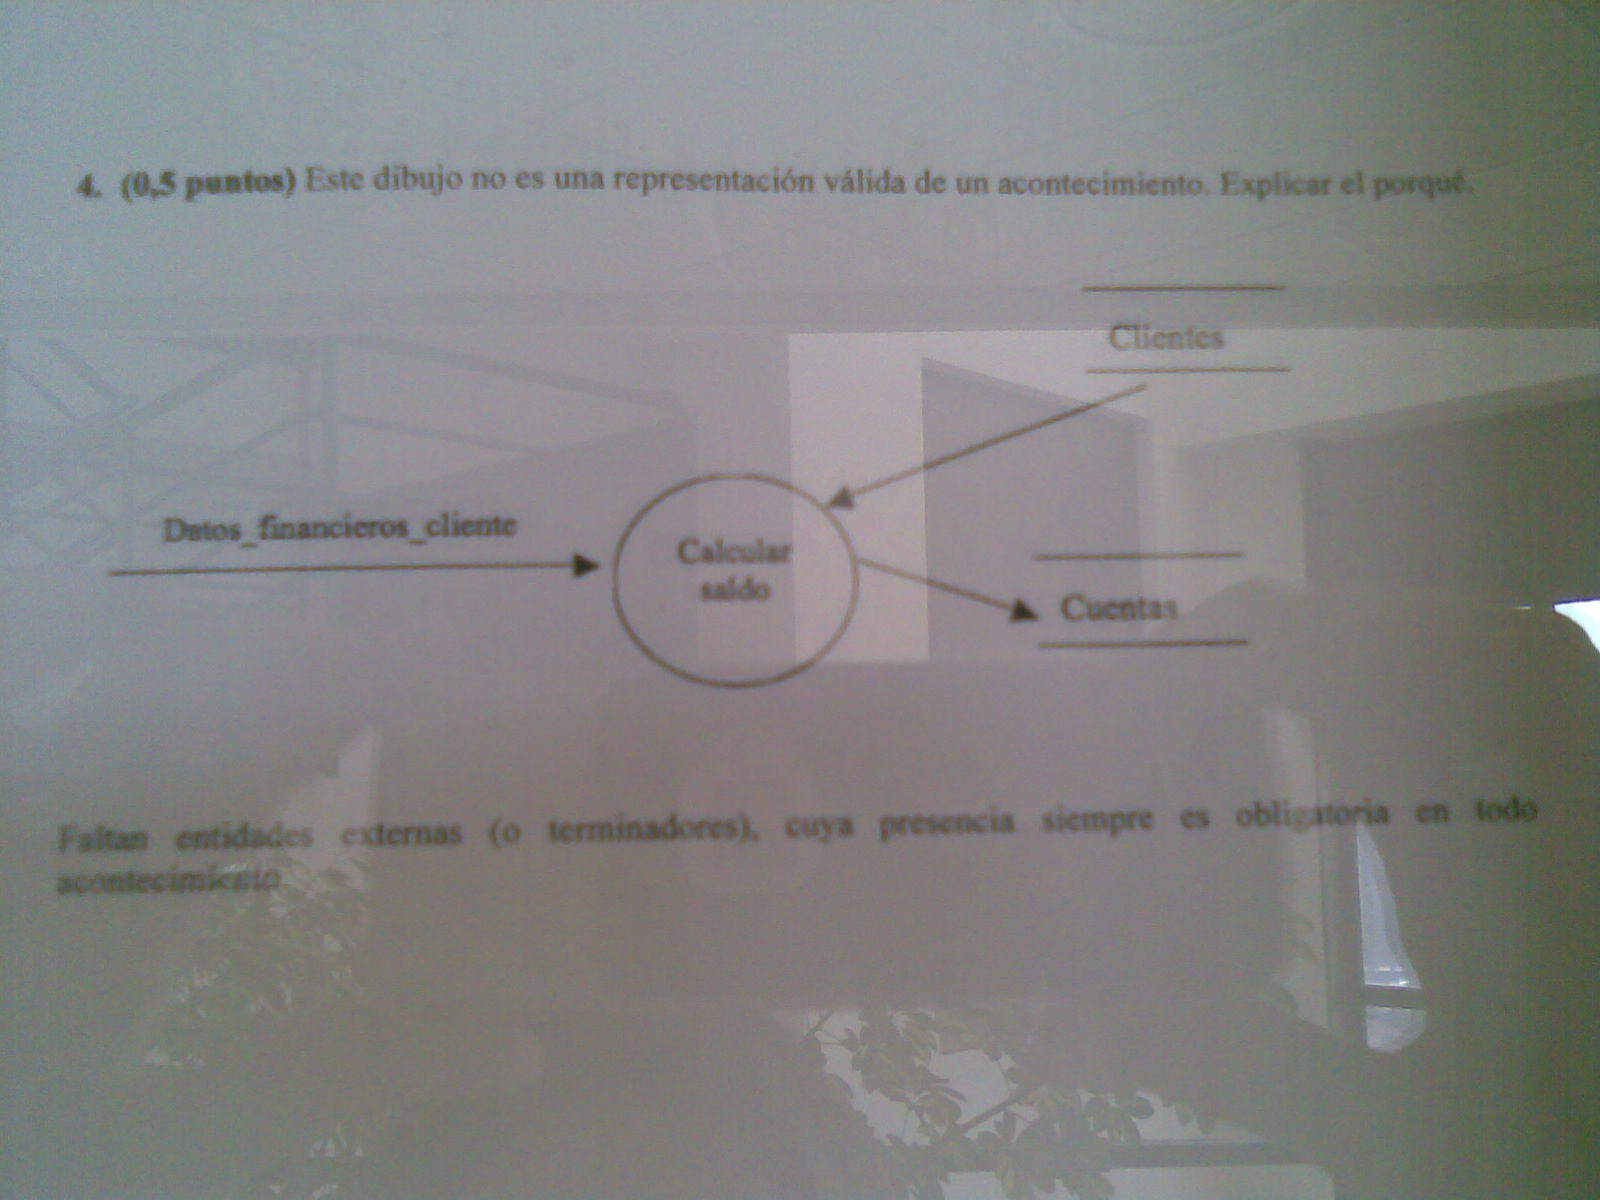
\includegraphics[width=\textwidth]{./images/jun/Imagen077.jpg}
\end{figure}
\begin{figure}
  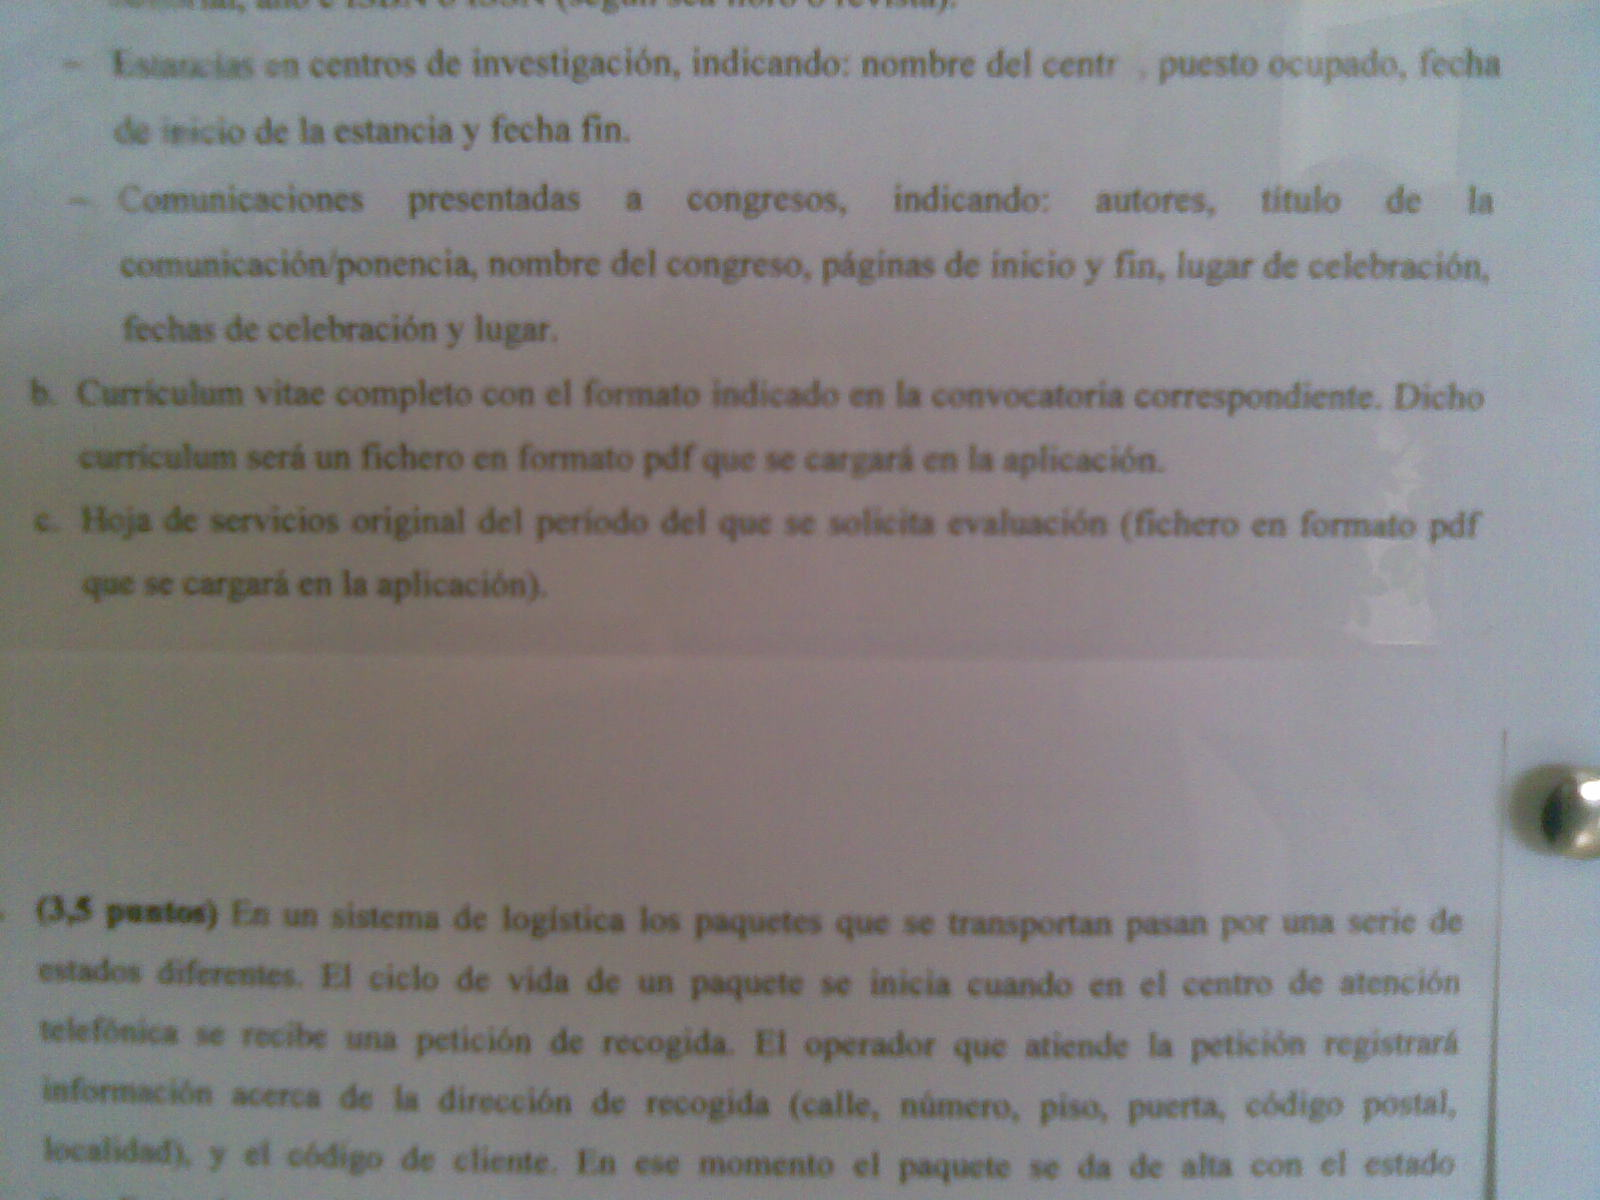
\includegraphics[width=\textwidth]{./images/jun/Imagen081.jpg}
\end{figure}
\begin{figure}
  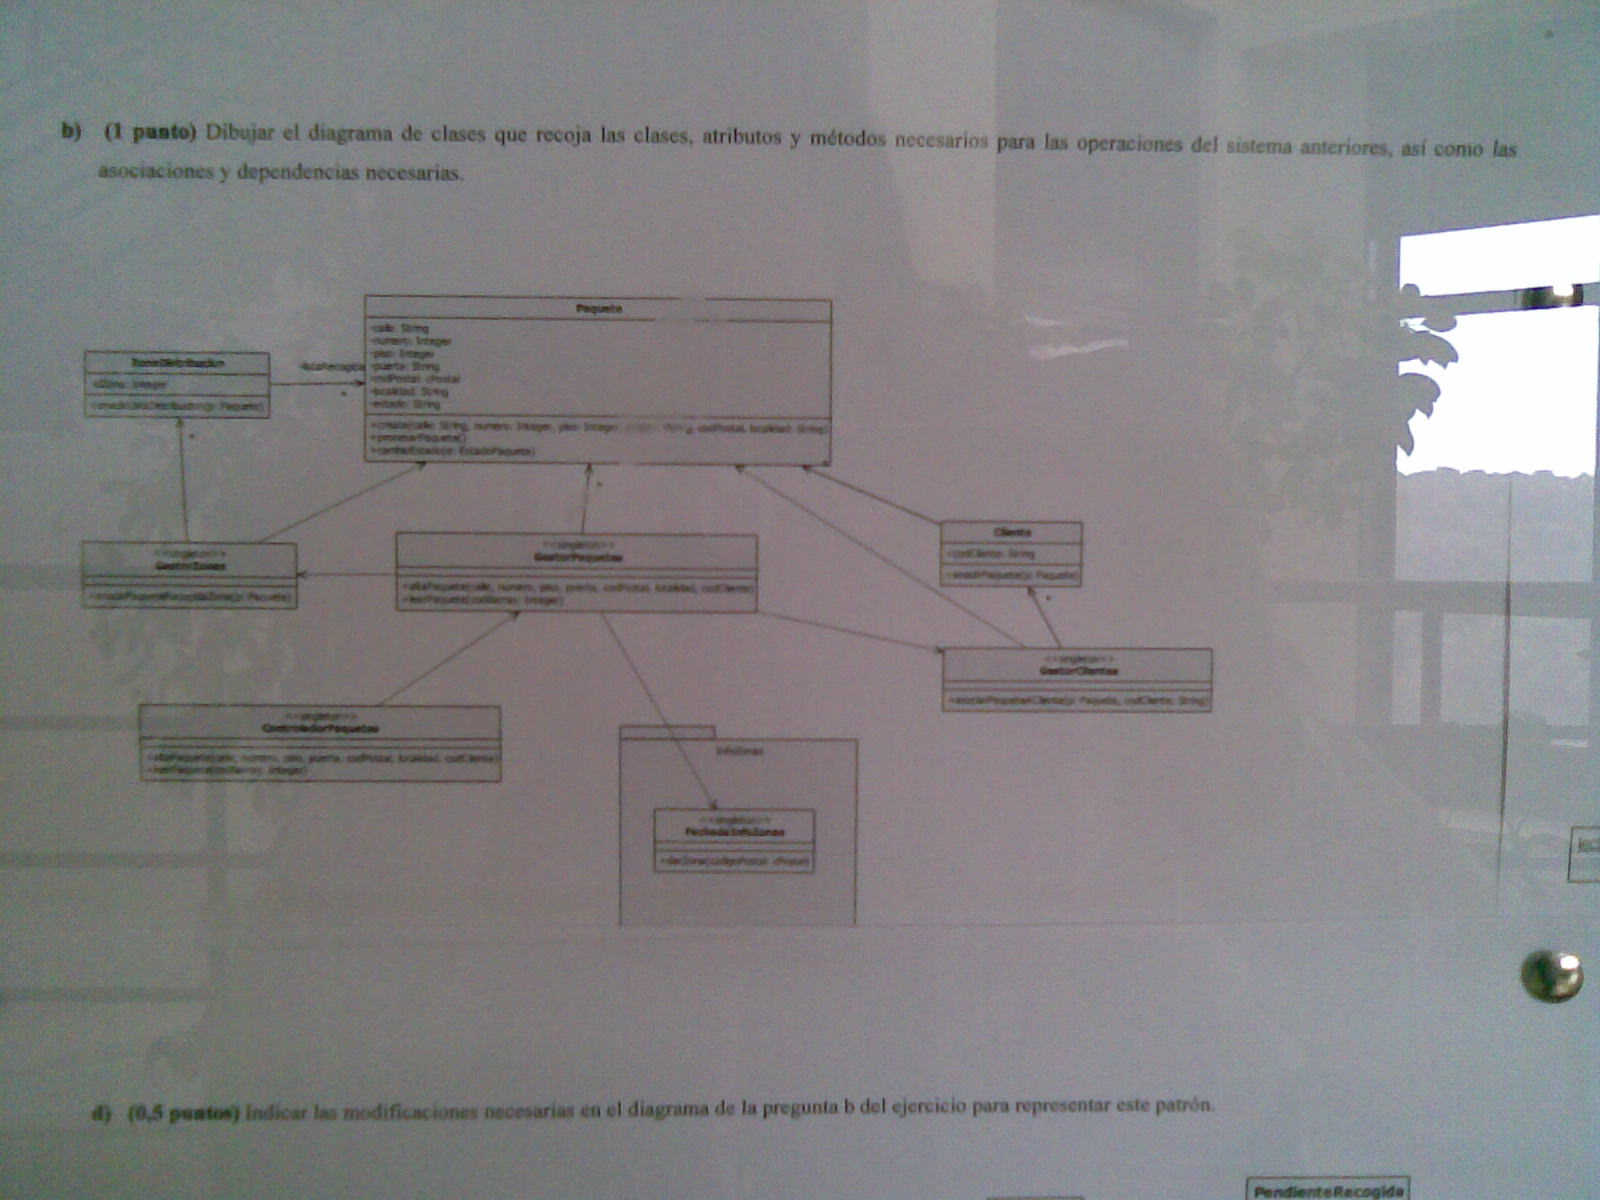
\includegraphics[width=\textwidth]{./images/jun/Imagen083.jpg}
\end{figure}
\begin{figure}
  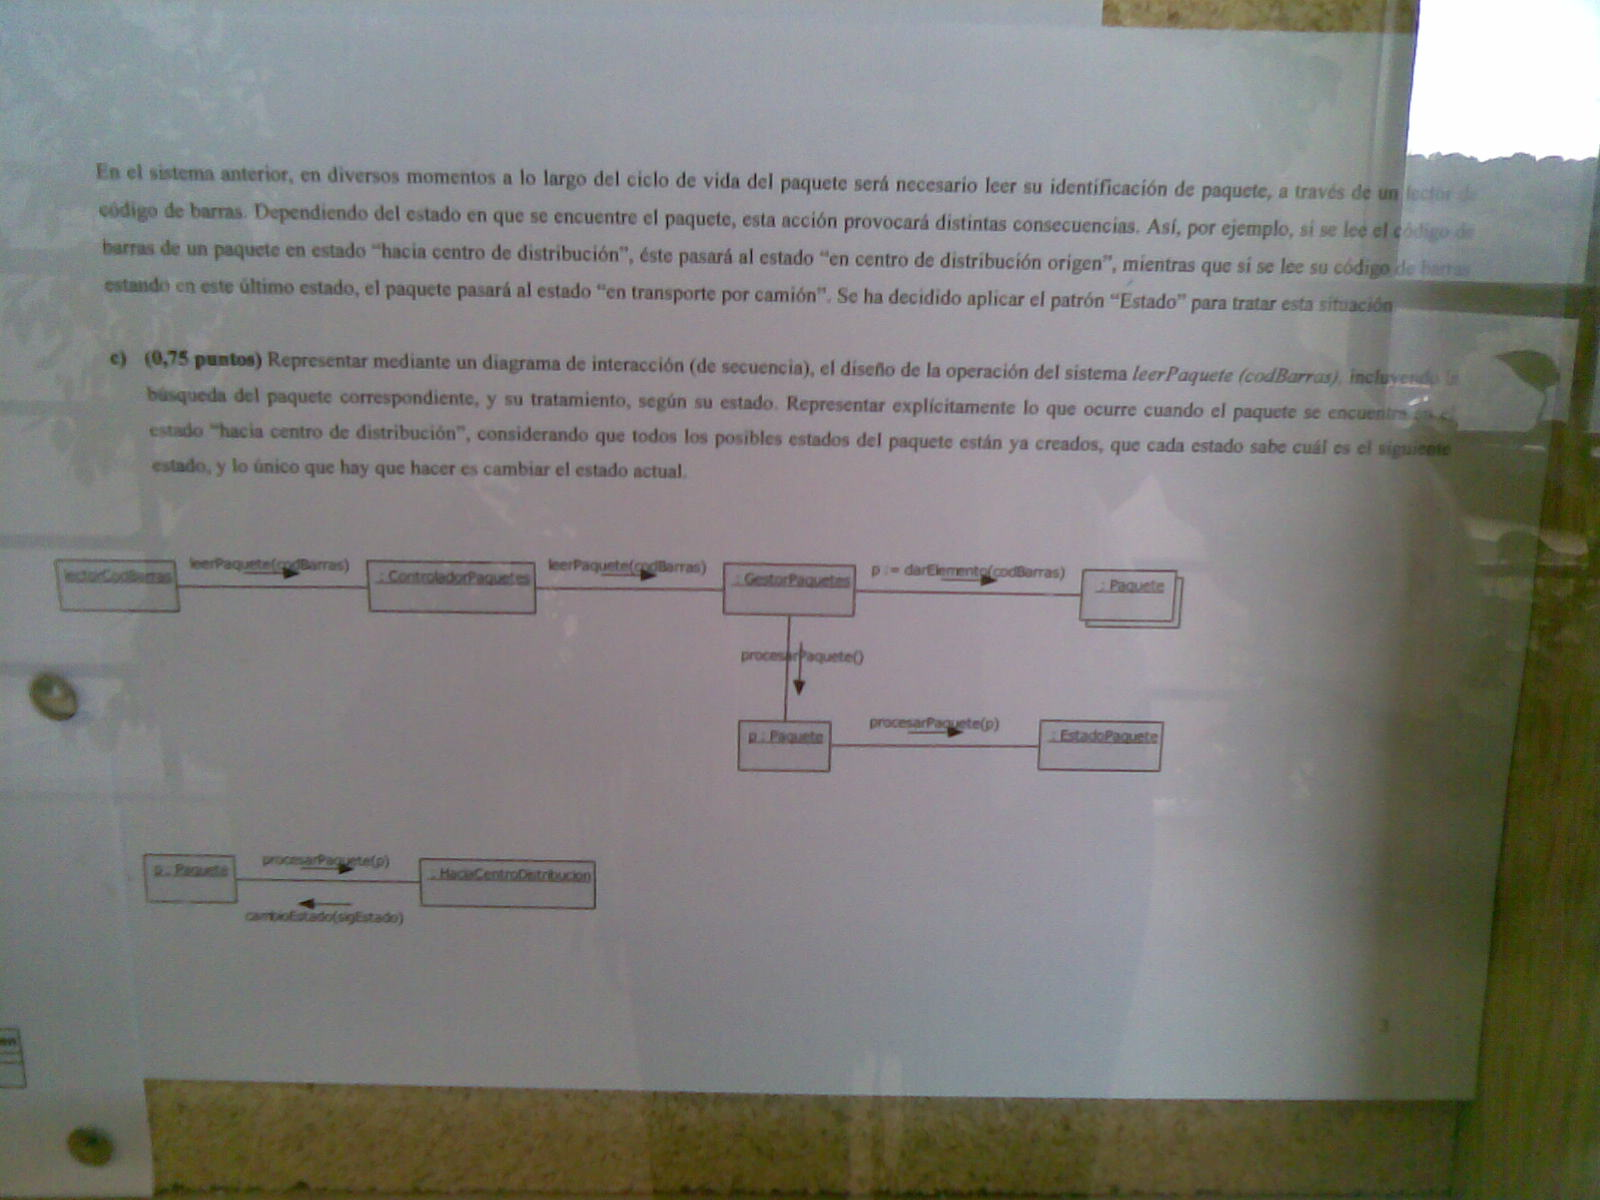
\includegraphics[width=\textwidth]{./images/jun/Imagen085.jpg}
\end{figure}
\begin{figure}
  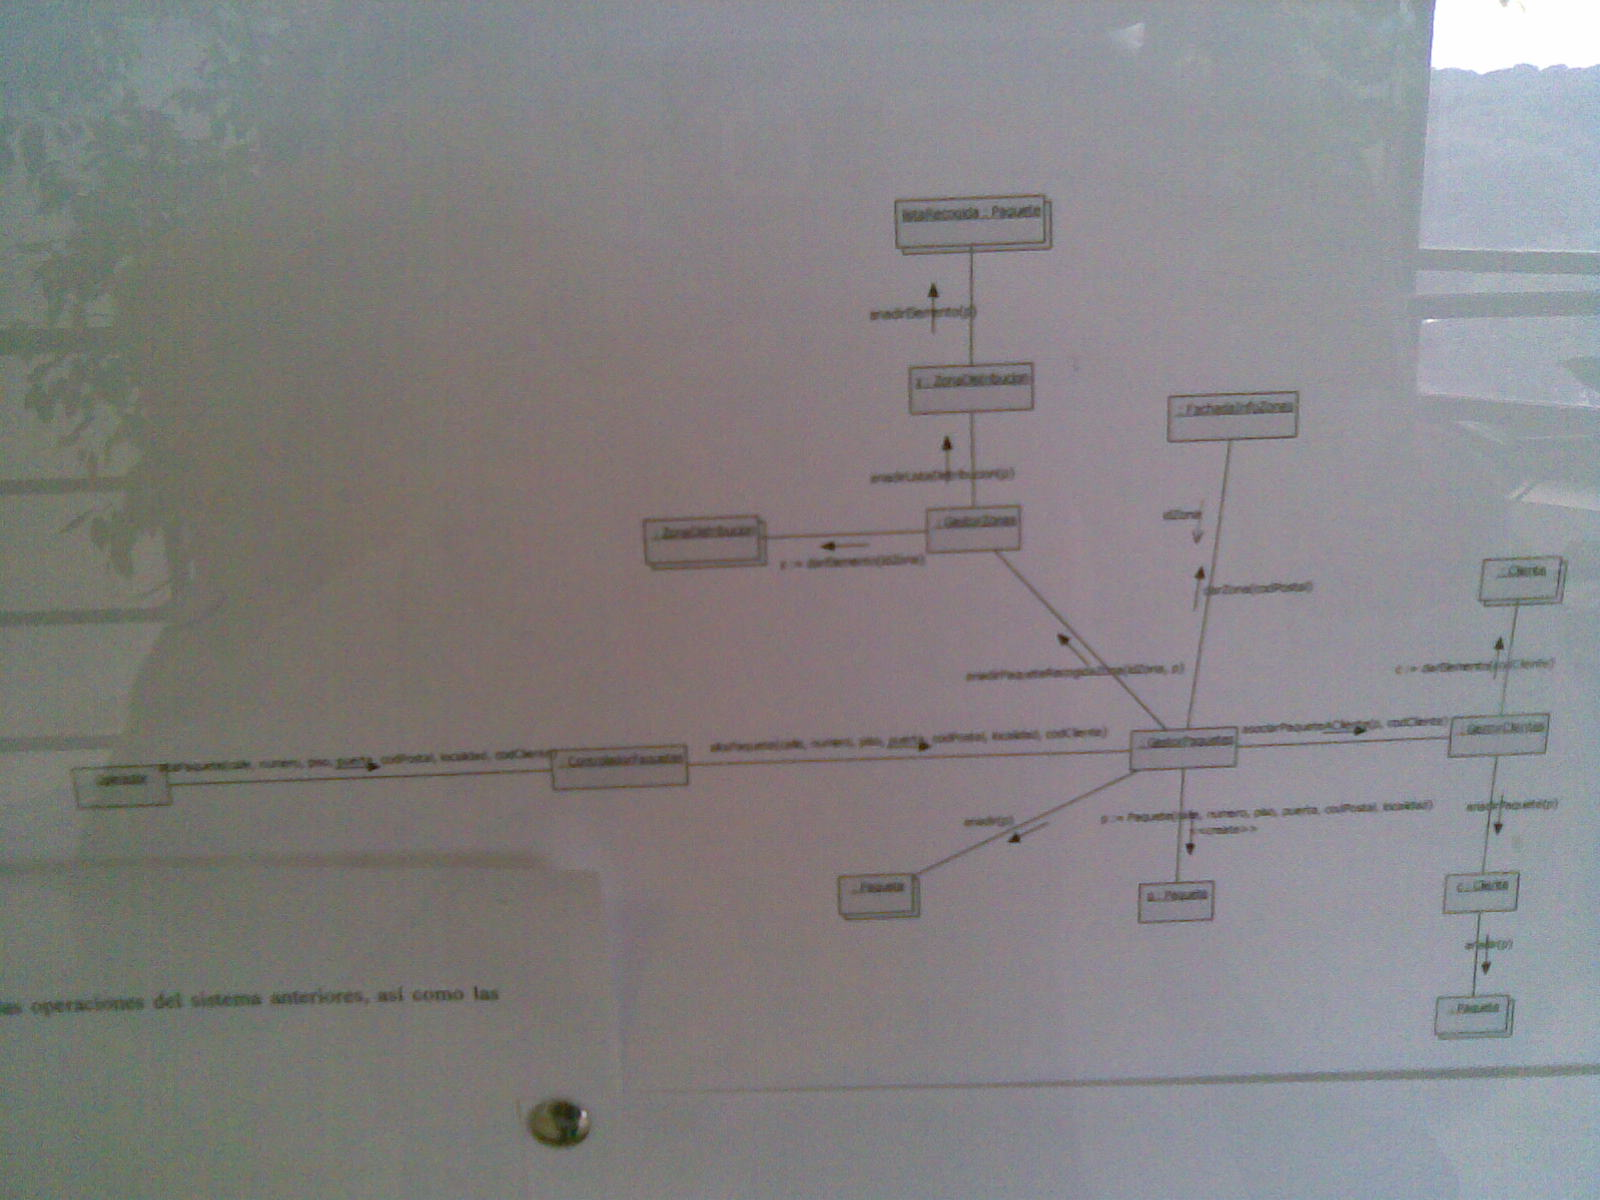
\includegraphics[width=\textwidth]{./images/jun/Imagen087.jpg}
\end{figure}
\begin{figure}
  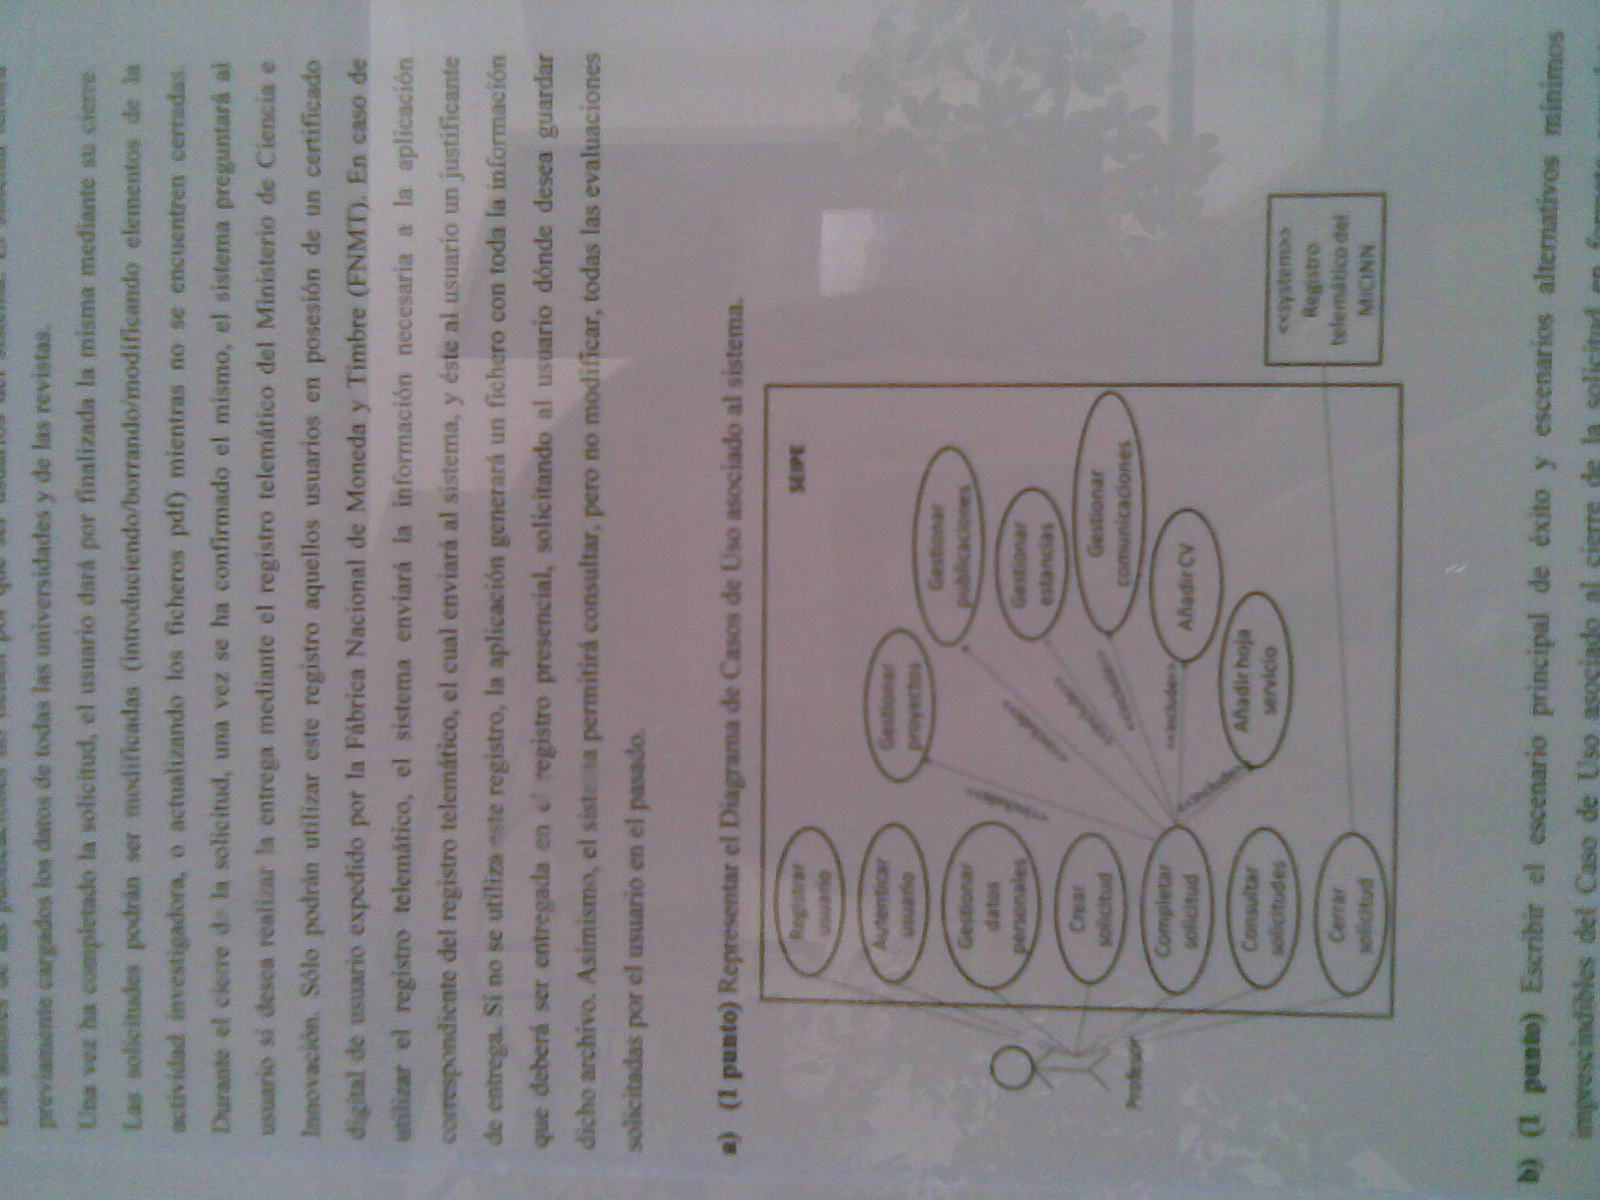
\includegraphics[width=\textwidth]{./images/jun/Imagen089.jpg}
\end{figure}
\begin{figure}
  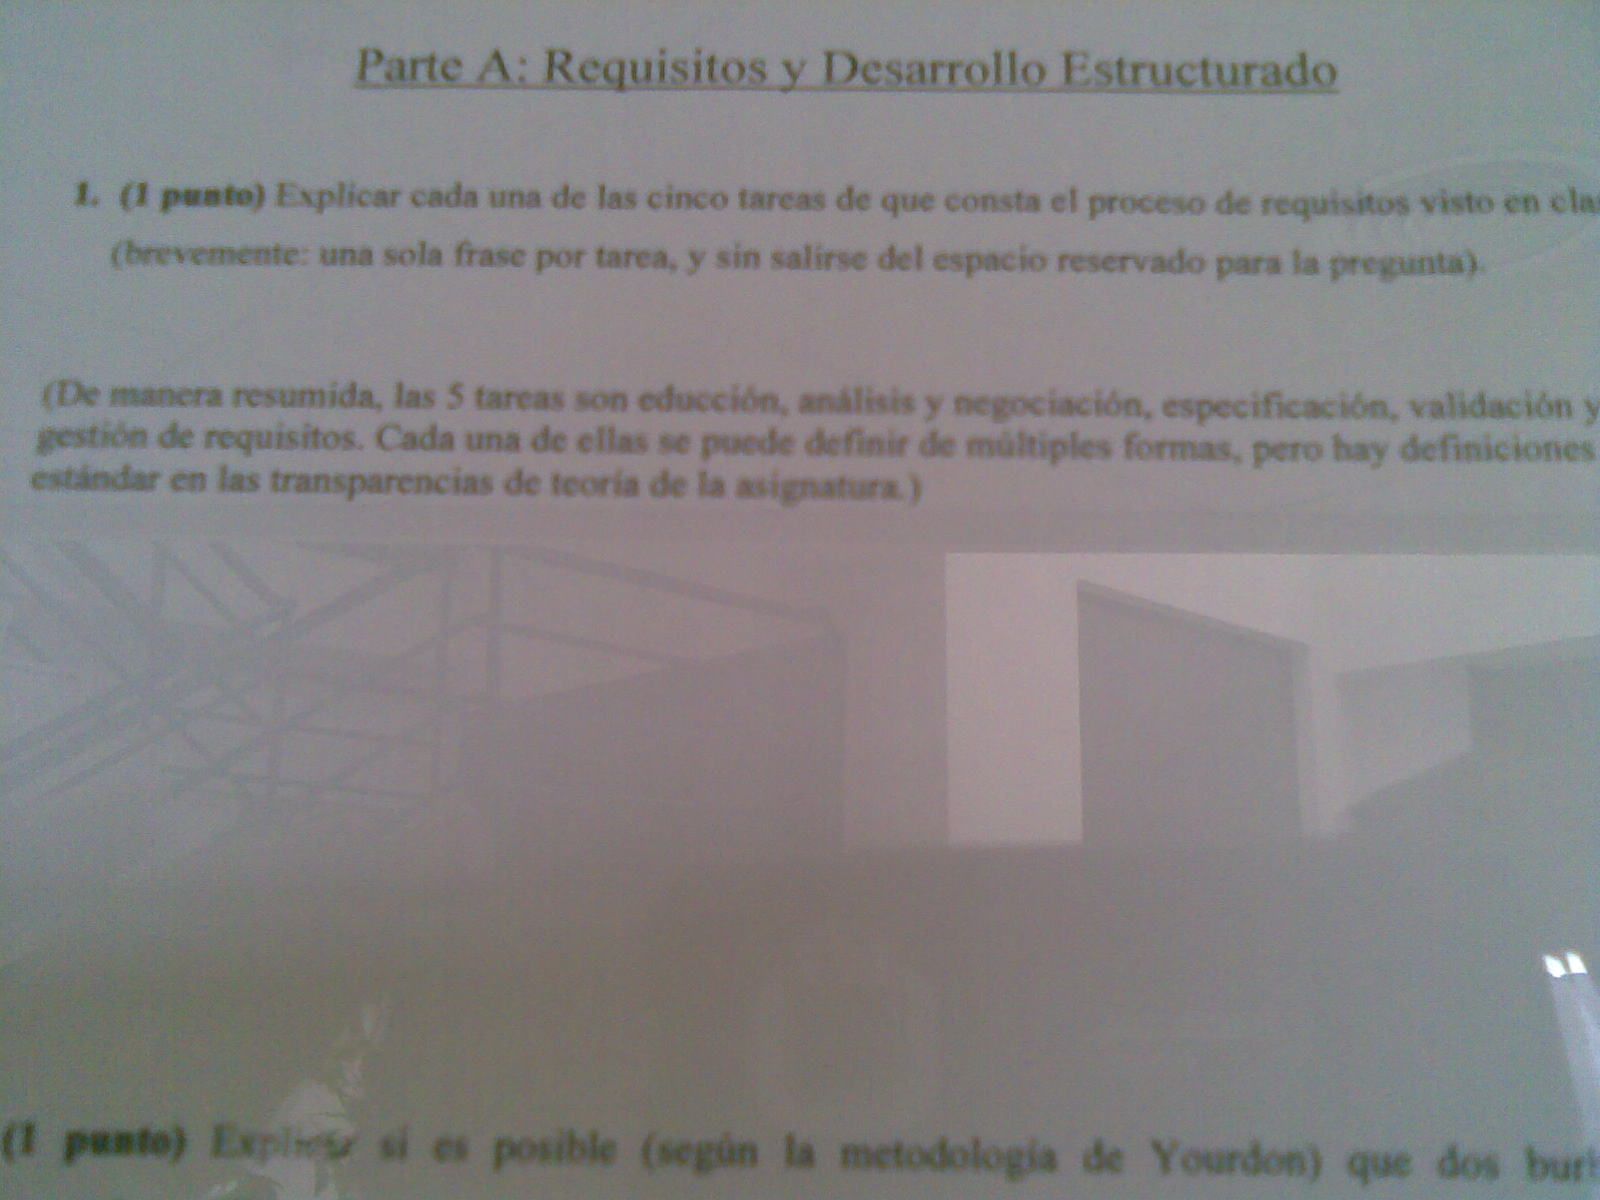
\includegraphics[width=\textwidth]{./images/jun/Imagen073.jpg}
\end{figure}
\begin{figure}
  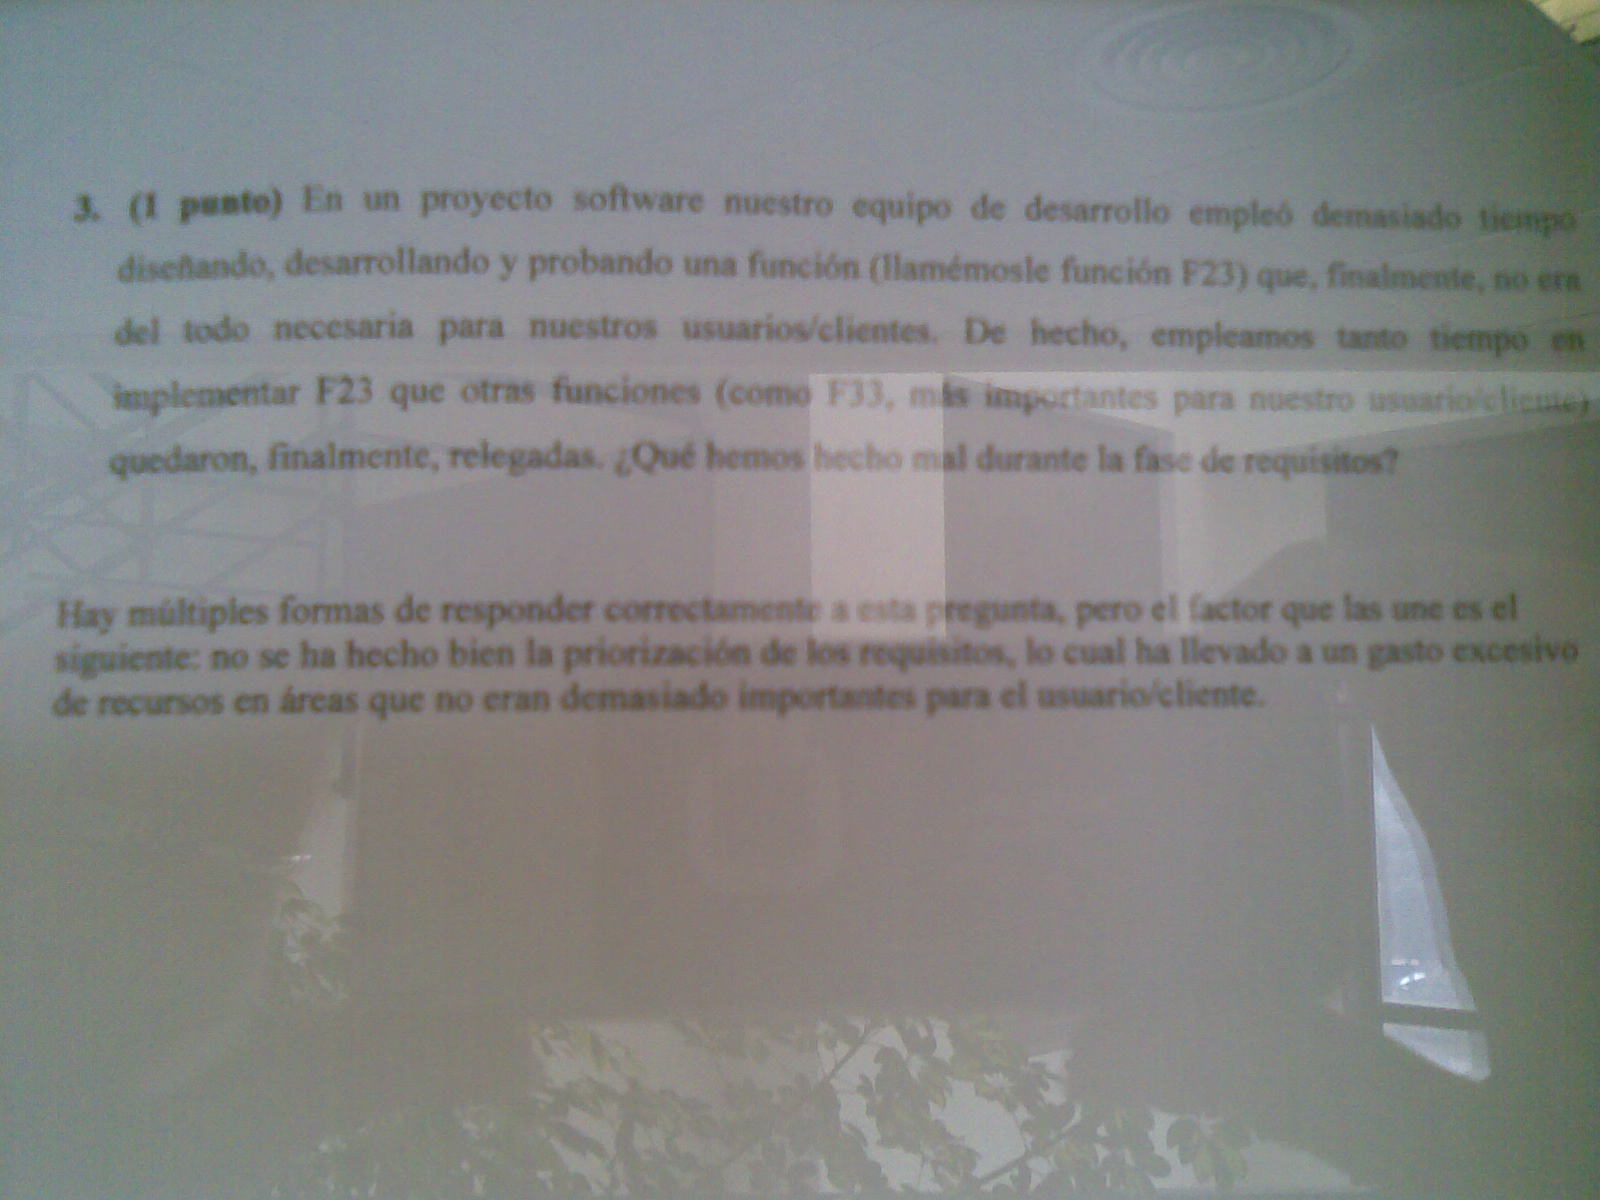
\includegraphics[width=\textwidth]{./images/jun/Imagen076.jpg}
\end{figure}
\begin{figure}
  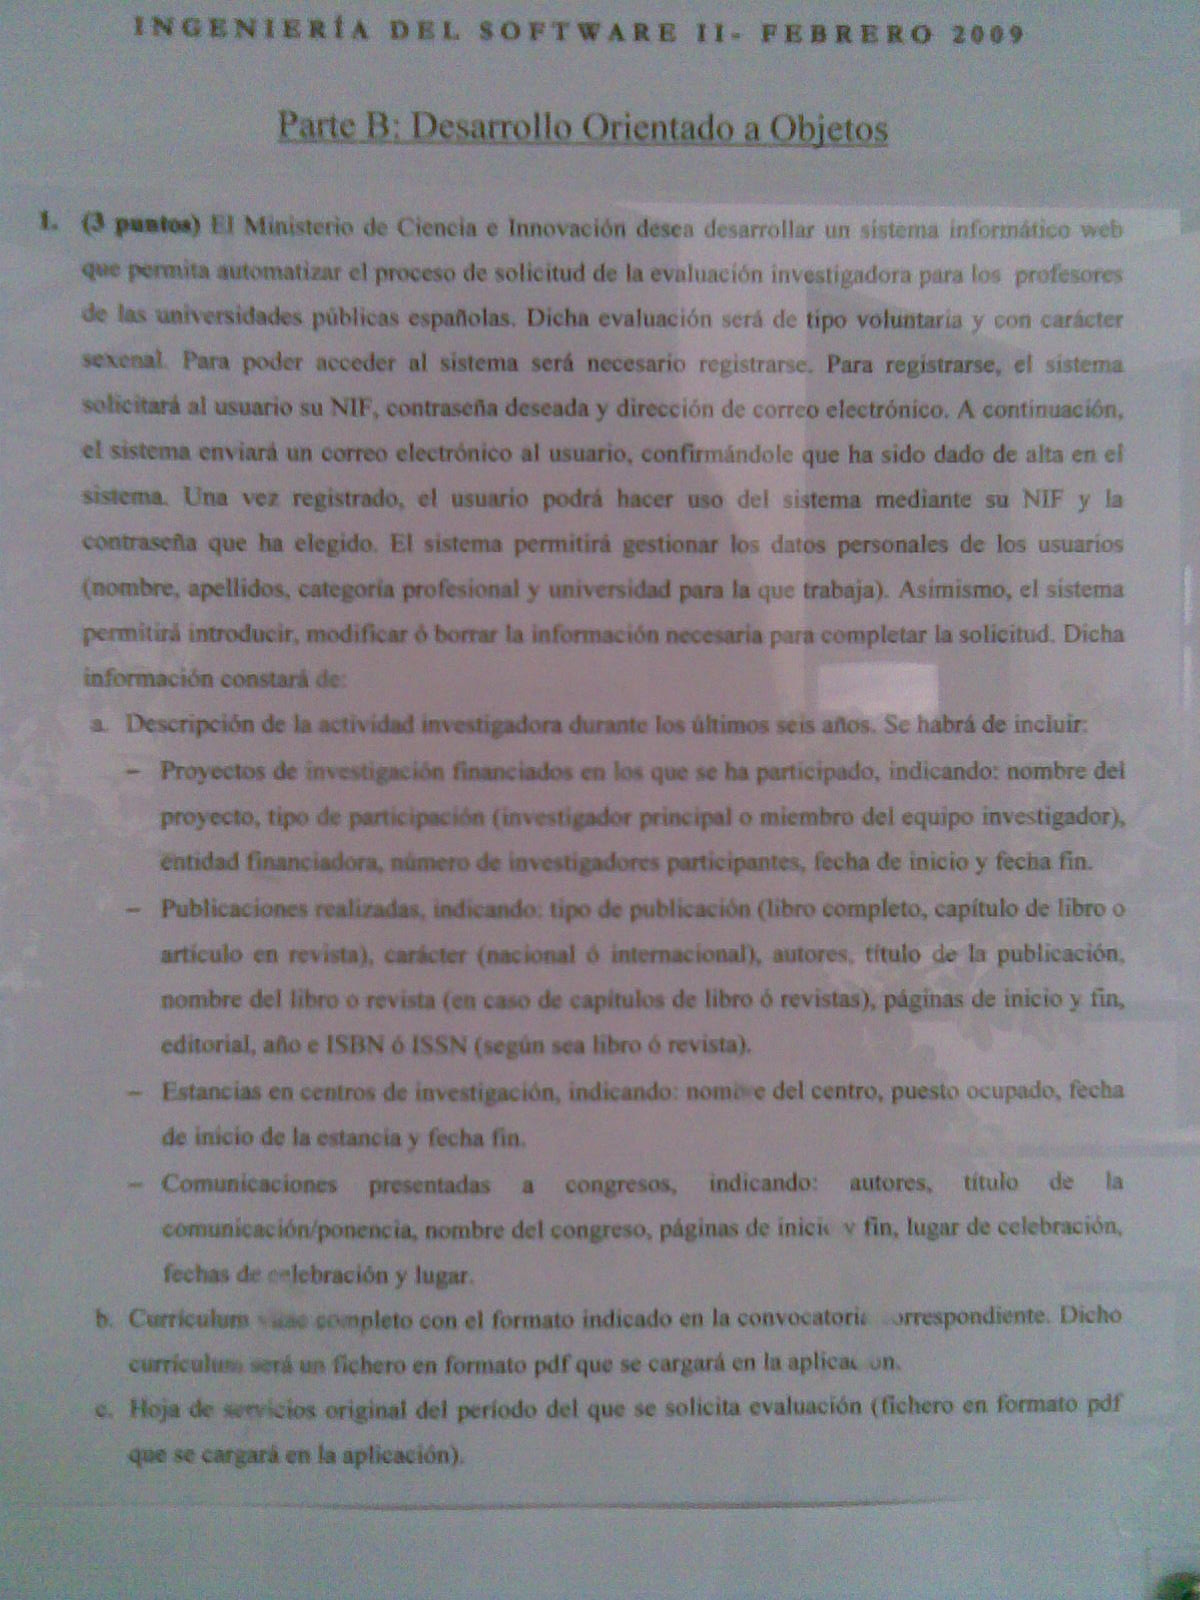
\includegraphics[width=\textwidth]{./images/jun/Imagen078.jpg}
\end{figure}
\begin{figure}
  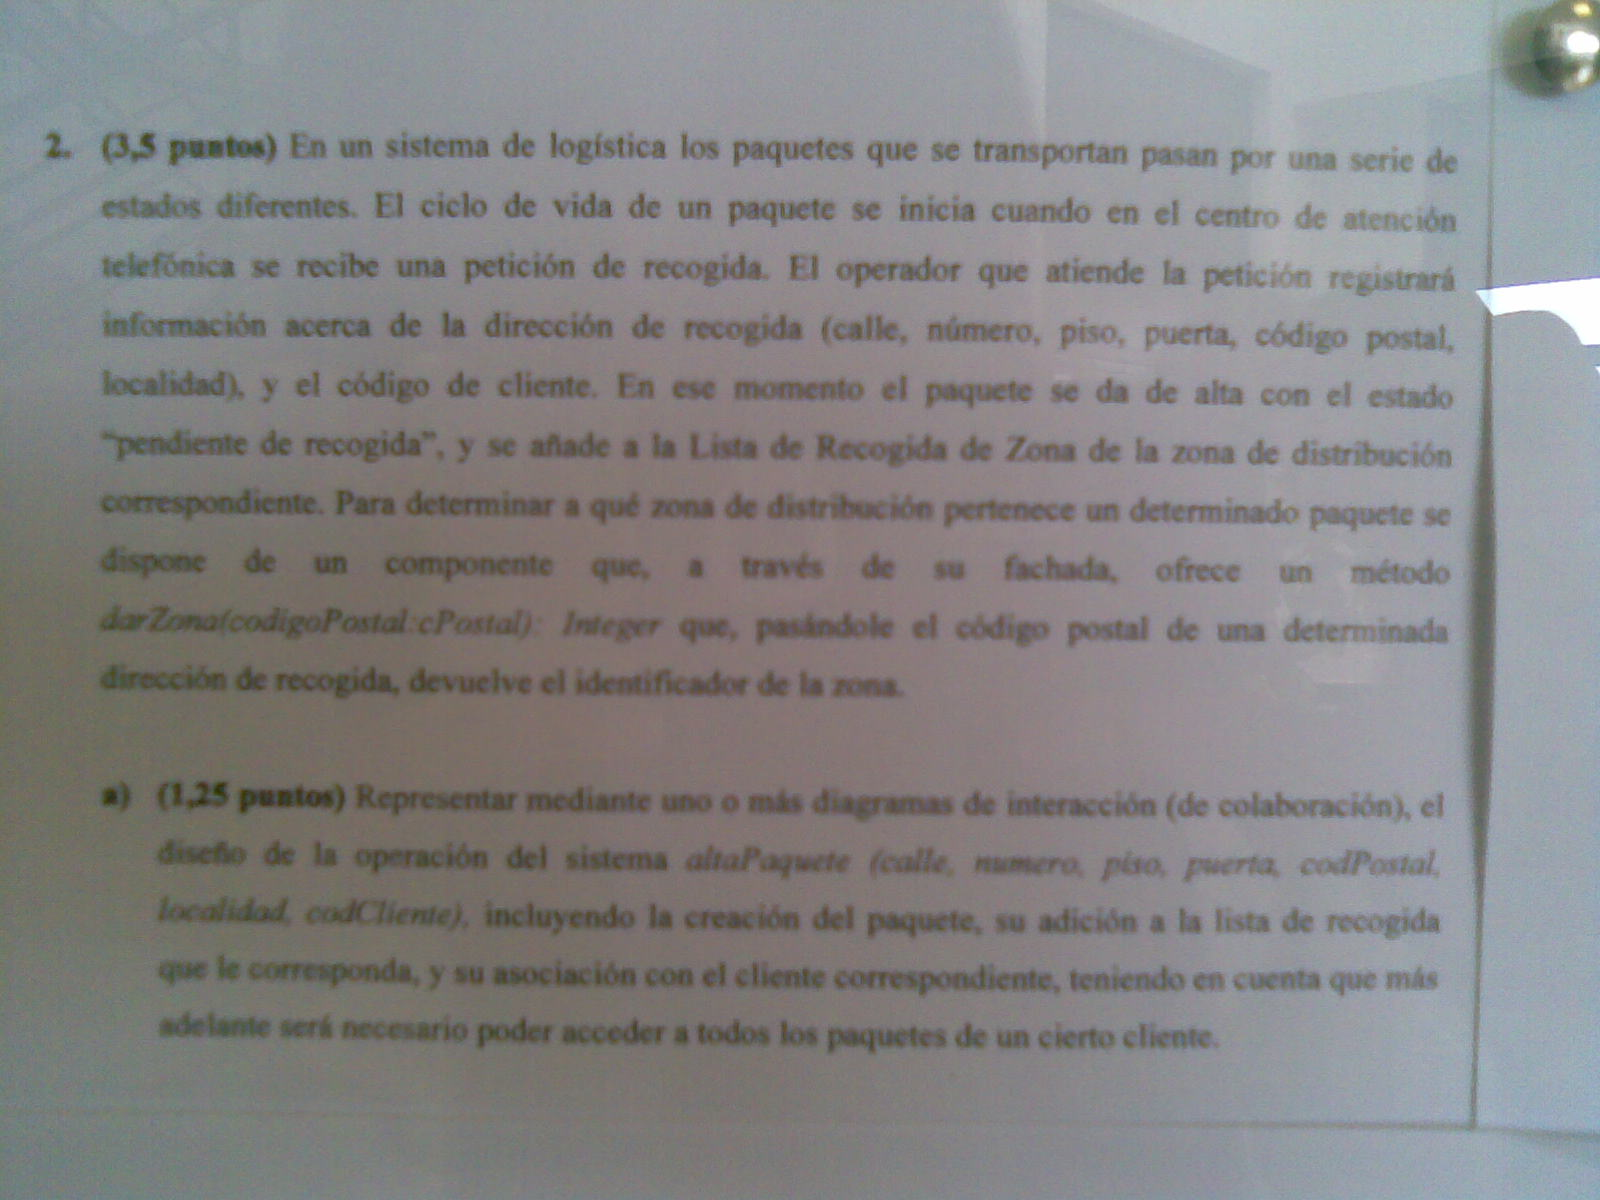
\includegraphics[width=\textwidth]{./images/jun/Imagen082.jpg}
\end{figure}
\begin{figure}
  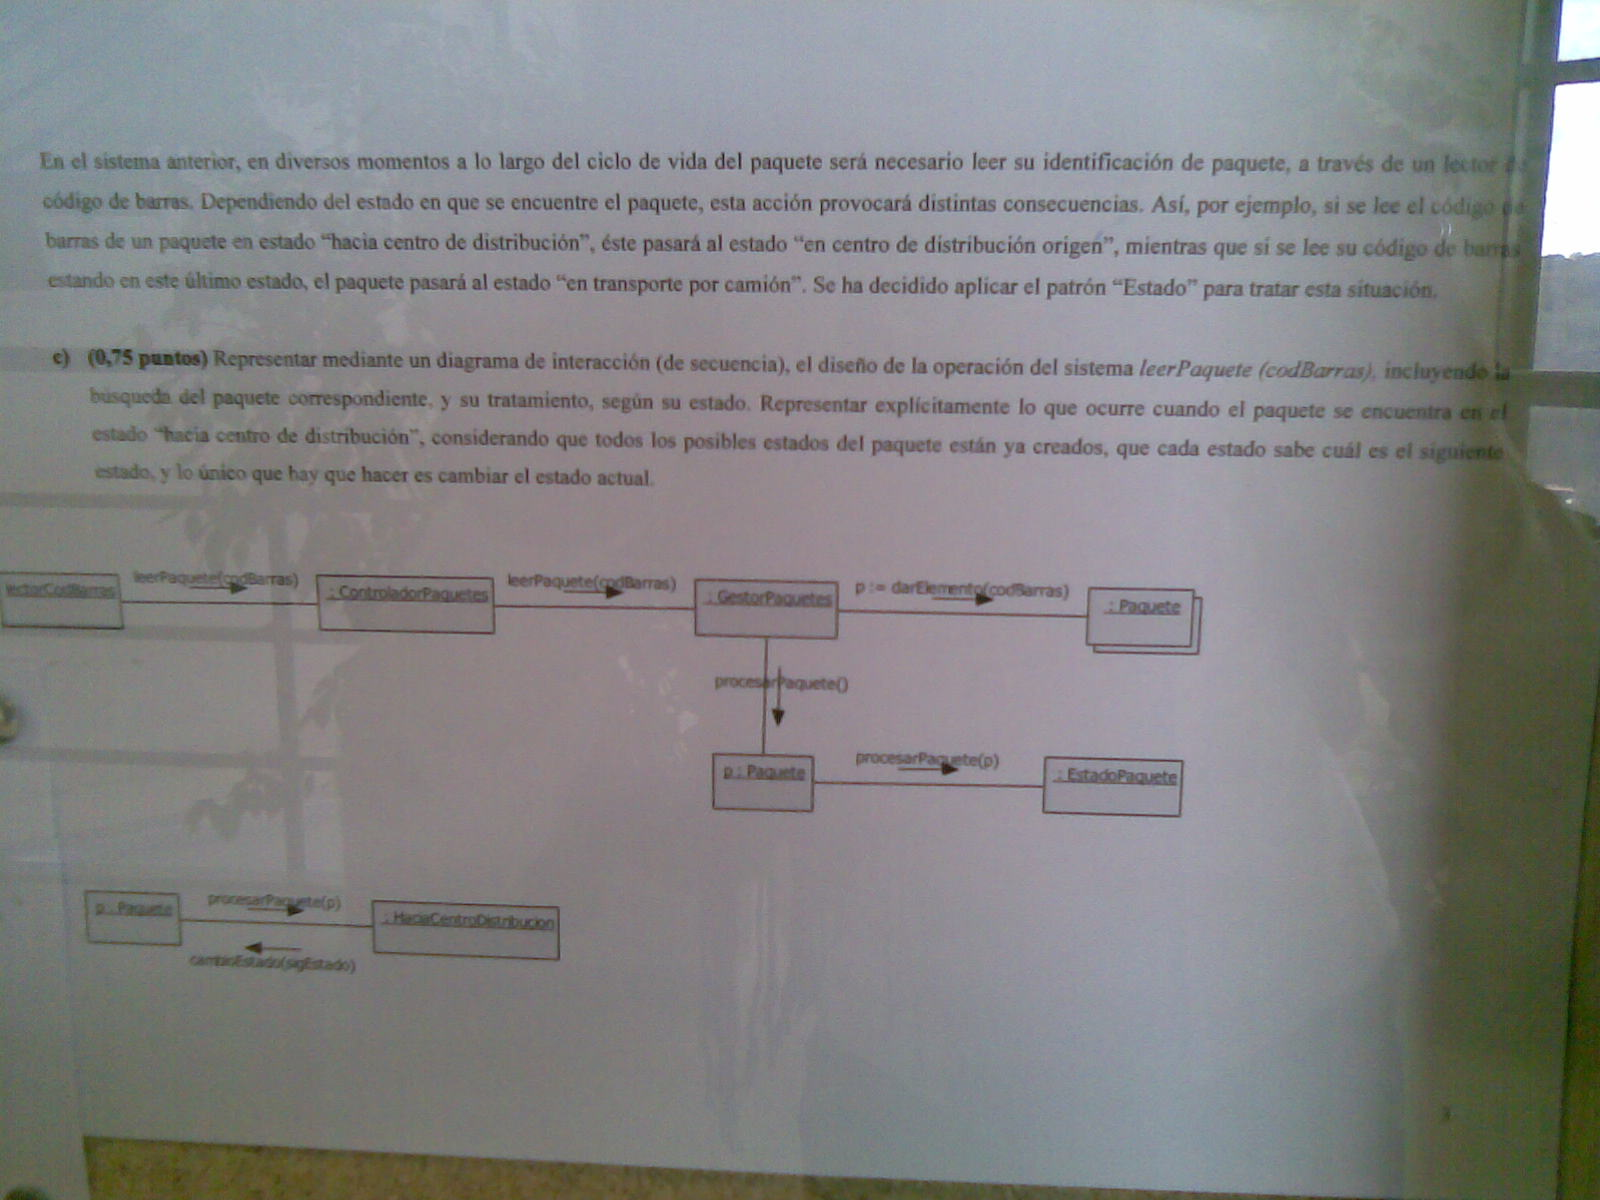
\includegraphics[width=\textwidth]{./images/jun/Imagen084.jpg}
\end{figure}
\begin{figure}
  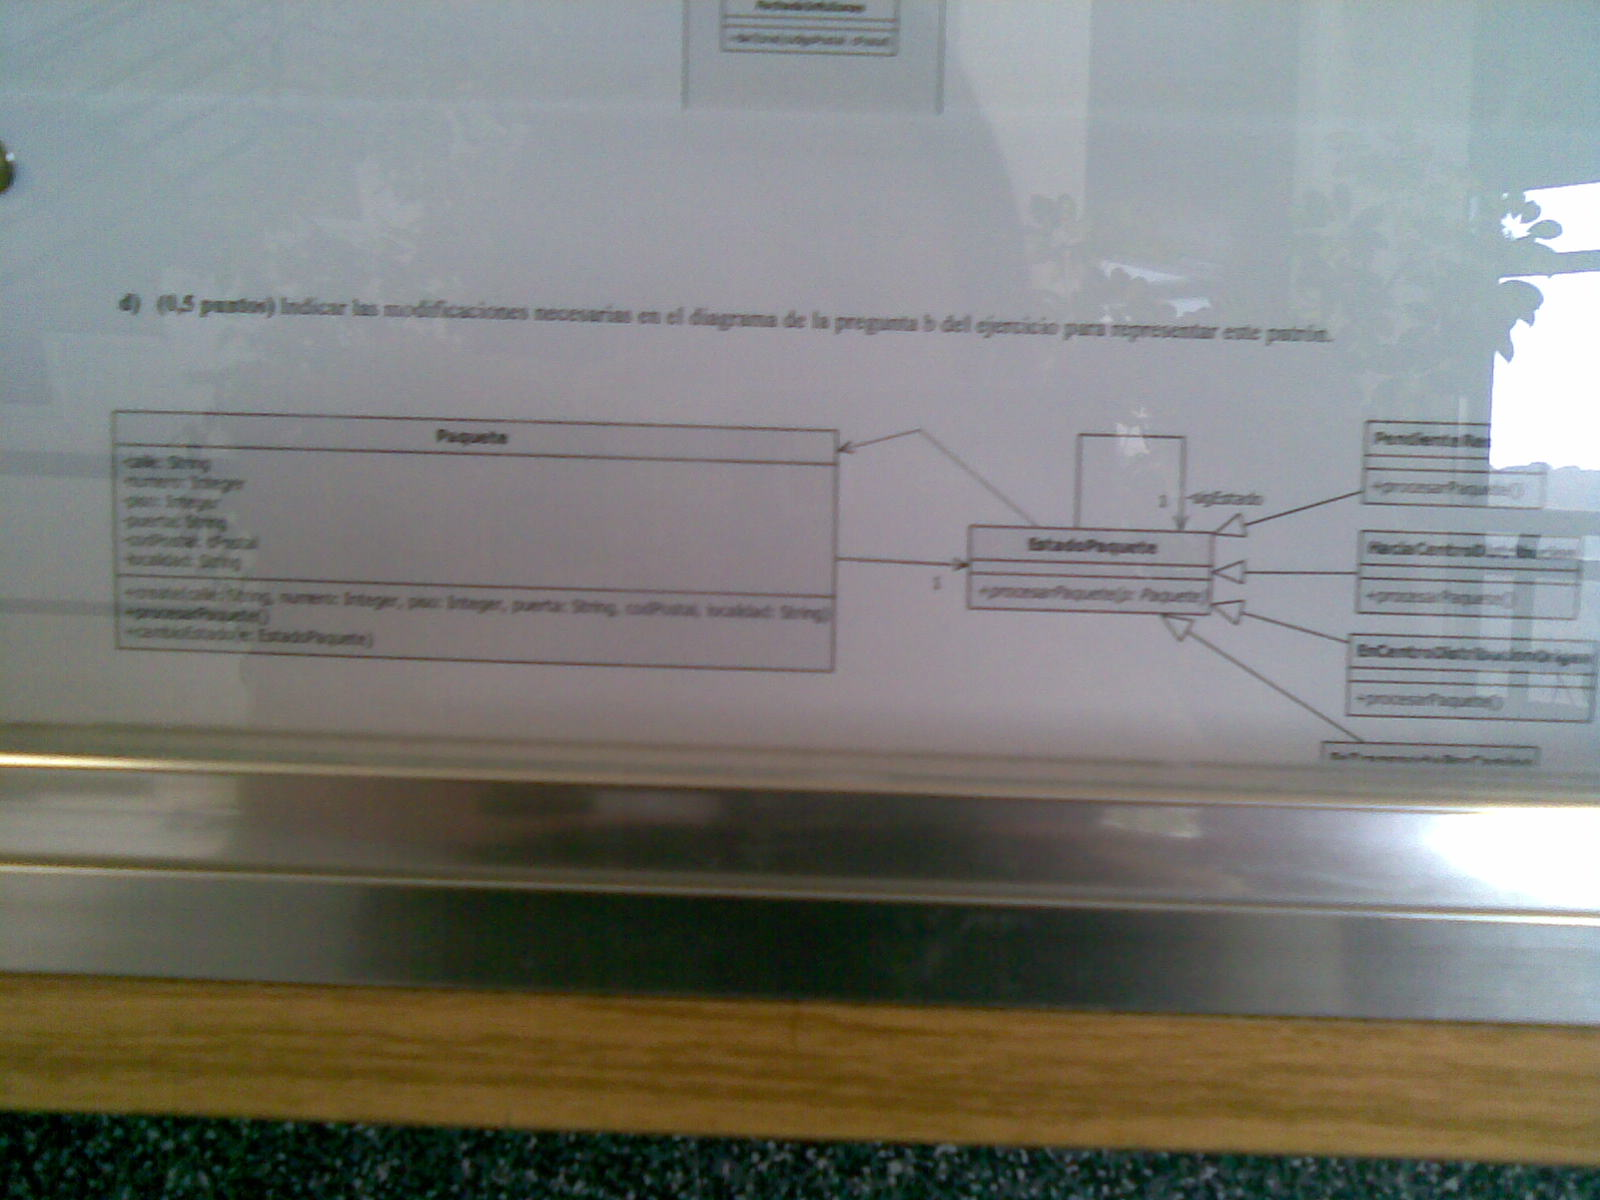
\includegraphics[width=\textwidth]{./images/jun/Imagen086.jpg}
\end{figure}
\begin{figure}
  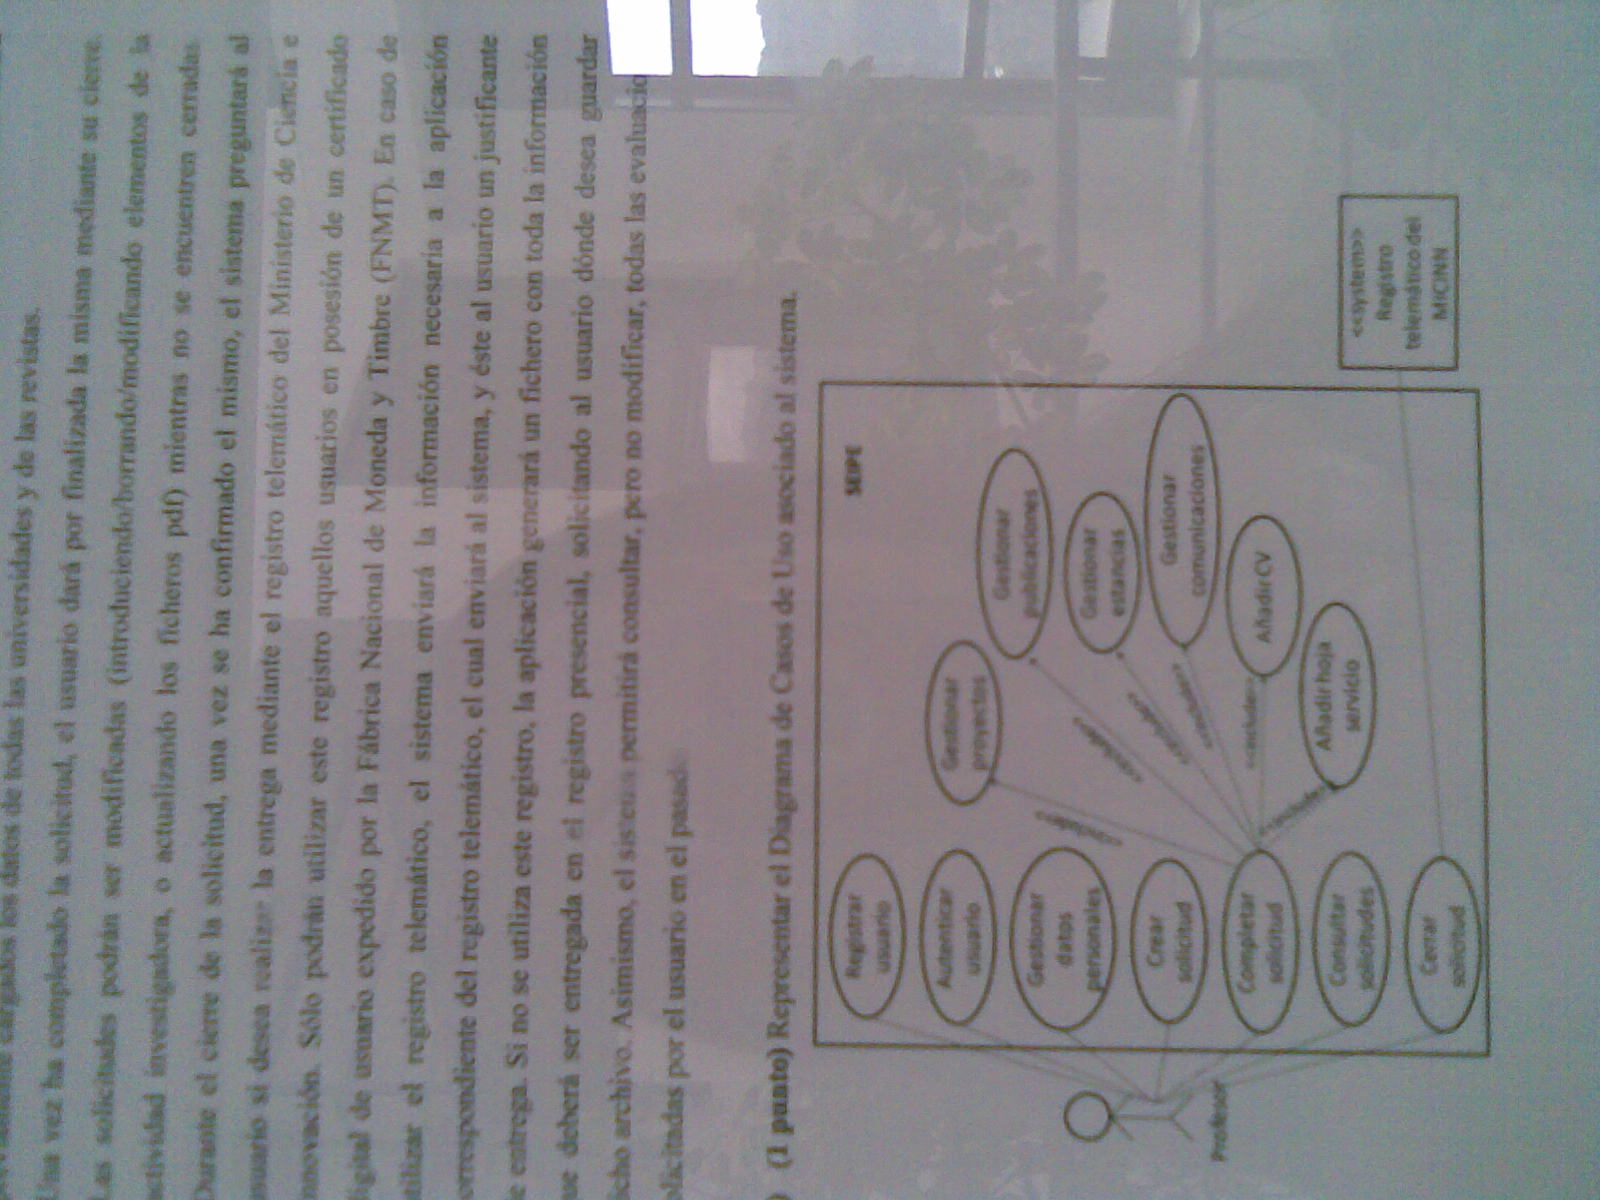
\includegraphics[width=\textwidth]{./images/jun/Imagen088.jpg}
\end{figure}
\begin{figure}
  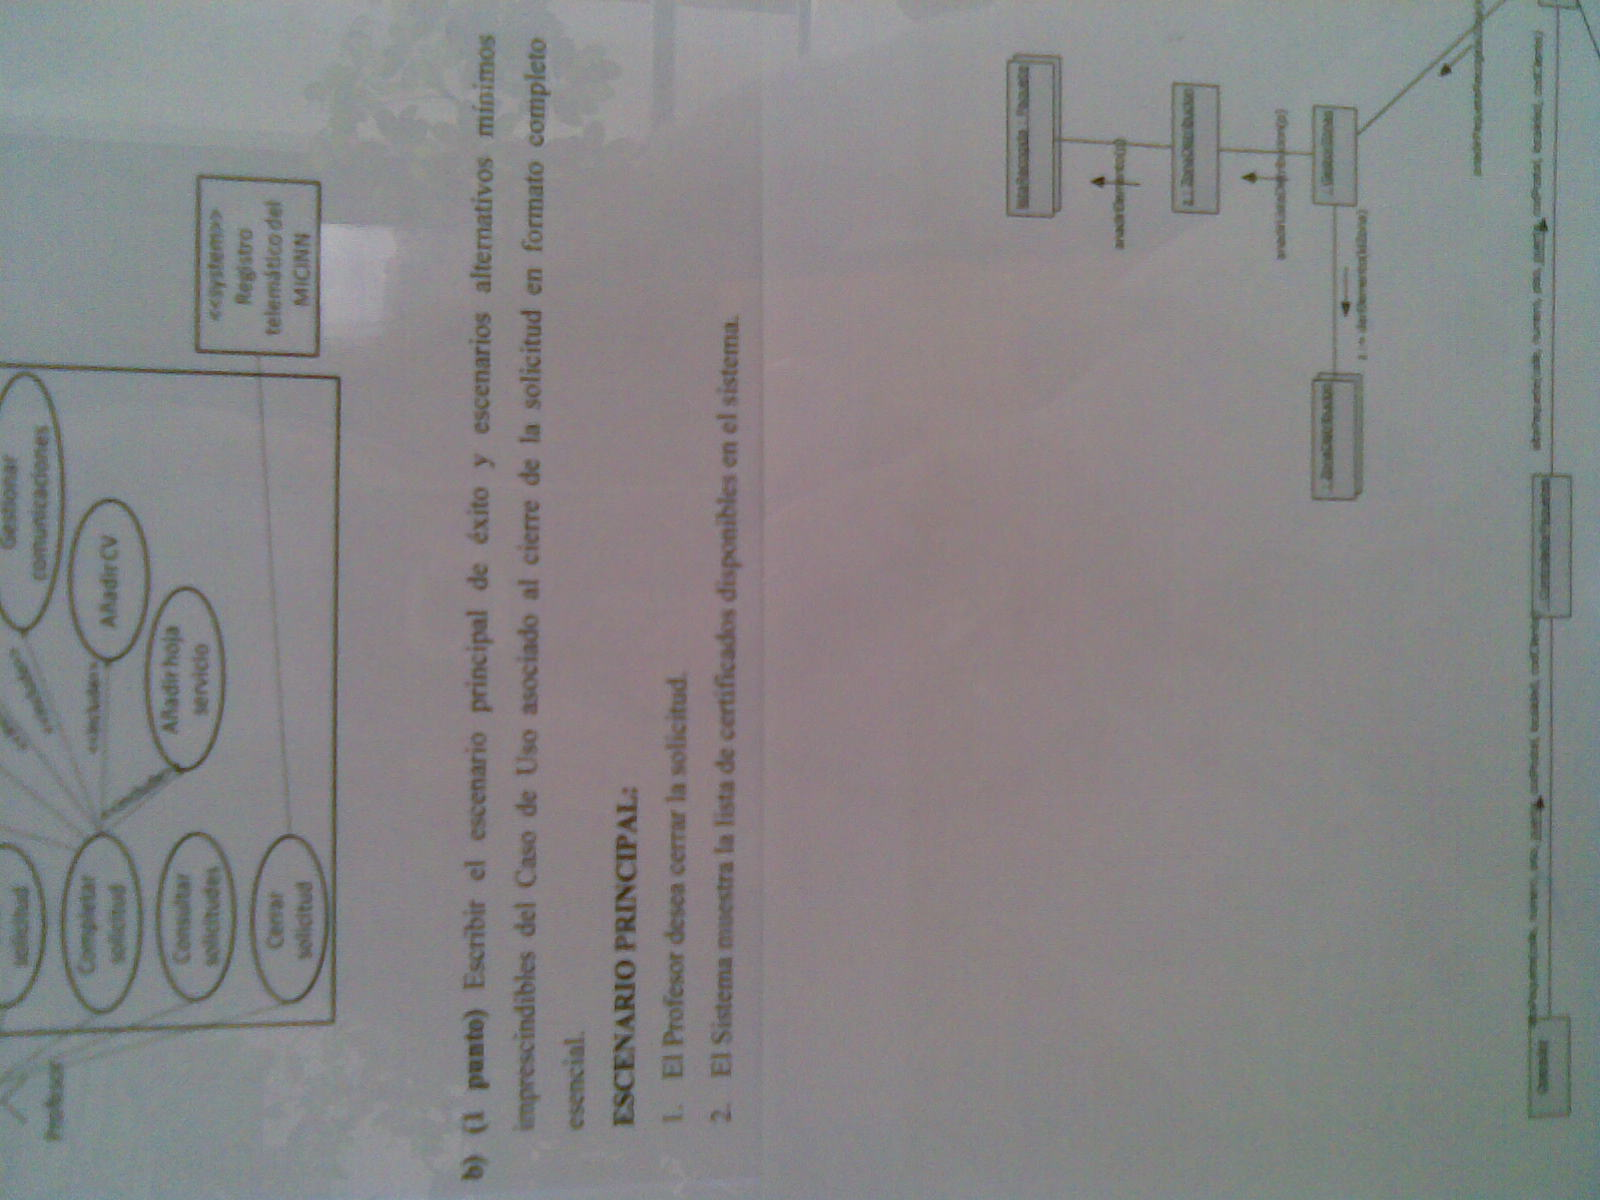
\includegraphics[width=\textwidth]{./images/jun/Imagen090.jpg}
\end{figure}


\bibliography{IS1apuntes}
\printindex
\end{document}
%%%%%%%%%%%%%%%%%%%%%%%%%%%%%%%%%%%%%%%%%%%%%

